% This must be in the first 5 lines to tell arXiv to use pdfLaTeX, which is strongly recommended.
\pdfoutput=1
% In particular, the hyperref package requires pdfLaTeX in order to break URLs across lines.

\documentclass[11pt]{article}

% Remove the "review" option to generate the final version.
\usepackage{acl}

% Standard package includes
\usepackage{times}
\usepackage{latexsym}

% For proper rendering and hyphenation of words containing Latin characters (including in bib files)
\usepackage[T1]{fontenc}
% For Vietnamese characters
% \usepackage[T5]{fontenc}
% See https://www.latex-project.org/help/documentation/encguide.pdf for other character sets

% This assumes your files are encoded as UTF8
\usepackage[utf8x]{inputenc}

% This is not strictly necessary, and may be commented out,
% but it will improve the layout of the manuscript,
% and will typically save some space.
\usepackage{microtype}

\usepackage{graphicx}
\usepackage{colortbl}
\usepackage{booktabs}
\usepackage{numprint}
\npthousandsep{\,}
\usepackage{tikz}
\usepackage{tablefootnote}

\newcommand{\fixme}[1]{\textbf{FIXME: {#1}}}
\newcommand{\ignore}[1]{}

%\usepackage[utf8x]{inputenc}

% English is the main language
\usepackage[thaicjk,english]{babel}
\addto\extrasthaicjk{\fontencoding{C90}\selectfont}

% Hack into CJKutf8 package for an option clash error
\makeatletter
\@namedef{opt@inputenc.sty}{utf8}
\makeatother
\usepackage{CJKutf8}
\usepackage[thaicjk,english]{babel}

%\usepackage{CJKutf8}
%\usepackage[english]{babel}
%\babelprovide[import]{thai} % Remove main if the main language is english
%\babelfont{rm}{FreeSerif}

% If the title and author information does not fit in the area allocated, uncomment the following
%
%\setlength\titlebox{<dim>}
%
% and set <dim> to something 5cm or larger.

\title{Aligning Word Vectors on Low-Resource Languages with Wiktionary}

% Author information can be set in various styles:
% For several authors from the same institution:
% \author{Author 1 \and ... \and Author n \\
%         Address line \\ ... \\ Address line}
% if the names do not fit well on one line use
%         Author 1 \\ {\bf Author 2} \\ ... \\ {\bf Author n} \\
% For authors from different institutions:
% \author{Author 1 \\ Address line \\  ... \\ Address line
%         \And  ... \And
%         Author n \\ Address line \\ ... \\ Address line}
% To start a seperate ``row'' of authors use \AND, as in
% \author{Author 1 \\ Address line \\  ... \\ Address line
%         \AND
%         Author 2 \\ Address line \\ ... \\ Address line \And
%         Author 3 \\ Address line \\ ... \\ Address line}

\author{Mike Izbicki \\
  Claremont McKenna College \\
  \texttt{mike@izbicki.me}}

\begin{document}
\maketitle
\begin{abstract}
    Aligned word embeddings have become a popular technique for low-resource natural language processing.
    Most existing evaluation datasets are generated automatically from machine translations systems,
    so they have many errors and exist only for high-resource languages.
    We introduce the Wiktionary bilingual lexicon collection,
    which provides high-quality human annotated translations for words in 298 languages to English.
    We use these lexicons to train and evaluate the largest published collection of aligned word embeddings on 157 different languages.
    All of our code and data is publicly available at \url{https://github.com/mikeizbicki/wiktionary_bli}.
    %most of which have never been previously aligned.
    %We identify 15 of these previously-unstudied languages (Armenian,
    %Austurian,
    %Azerbaijani,
    %Basque,
    %Belarusian,
    %Esperanto,
    %Galician,
    %Georgian,
    %Malayalam,
    %Norwegian Nynorsk,
    %Serbo-Croatian/sr,
    %Serbo-Croatian/sh,
    %and Welsh)
    %as having surprisingly good performance on the lexicon induction task suggesting that they may be suitable for zero-shot learning on downstream tasks.
\end{abstract}

%%%%%%%%%%%%%%%%%%%%%%%%%%%%%%%%%%%%%%%%%%%%%%%%%%%%%%%%%%%%%%%%%%%%%%%%%%%%%%%%

\section{Introduction}

A bilingual lexicon is a mapping of words from a source language into a target language.
The \emph{bilingual lexicon induction} (BLI) problem is the task of learning such a mapping from data.
Most recent solutions to this problem follow a two step procedure:
First, train word vectors on a large monolingual corpus for each language individually using a standard algorithm like word2vec \citep{mikolov2013efficient}, GloVe \cite{pennington2014glove}, or fastText \citep{bojanowski2017enriching}.
Then, learn a transformation that aligns these two vector spaces into a common space \citep[e.g.][]{mikolov2013exploiting,xing2015normalized,joulin2018loss,artetxe2018generalizing,zhang2019girls,glavas2019properly,vulic2019we}.
%\fixme{more cites}
The BLI problem is then solved by performing nearest neighbor queries in the common space.
The focus of this work is the ground truth bilingual lexicon used to train and evaluate these models.

Recent previous work has relied on the MUSE lexicon collection \citep{conneau2017word}.
This collection provides bilingual lexicons between 45 languages and English.
%and a small number of bilingual lexicons between high-resource non-English language pairs.
This lexicon is generated from a machine translation system,
and so suffers from a number of problems.
First, many of the mappings in the lexicon do not contain real words in either the source or target language
(see Figure \ref{fig:th-vi} for examples from Thai).
Second, the distribution of words is inconsistent between languages,
with many languages containing only proper nouns in their training and test sets.
Due to these problems, \citet{kementchedjhieva2019lost} suggest that future research ``avoids drawing conclusions from quantitative results on this BLI dataset.''
Other datasets (described in Section \ref{sec:related-work} below) have even worse limitations.

This paper introduces a new bilingual lexicon collection based on Wiktionary.
Wiktionary contains more than 7 million words in 8166 languages and has been collaboratively edited by 3.9 million users.%
\footnote{\url{https://en.wiktionary.org/wiki/Wiktionary:Statistics}}
%Each word in Wiktionary is annotated with a part of speech tag and at least one English language definition.
%\footnote{\url{https://wiktionary.com}}.
%Our collection solves the existing problems with the MUSE collection and greatly extends the language coverage.
%Wiktionary is a large and publicly editable dictionary,
%similar to how Wikipedia is a large publicly editable encyclopedia.
%We use the English-language Wiktionary dump from 1 July 2022\
%\footnote{Available form \url{https://en.wiktionary.org/wiki/Help:FAQ\#Downloading_Wiktionary}}
%.
Our specific contributions are:
\begin{enumerate}
    \item
        We use Wiktionary to construct high-quality bilingual lexicons suitable for training and evaluating BLI models from 298 languages into English.
        Most of these languages are extremely low-resource,
        and many of them are extinct. % (e.g.\ Ancient Greek, Old English, Tocharian B).
        We provide the first BLI datasets for 253 of these languages,
        and for the remaining 45 we improve the quality of existing datasets.
        Our lexicon collection is the first to allow meaningful cross-lingual performance comparisons on the BLI task.
        %The datasets and code for generating them are publicly available on github.\footnote{URL blinded for review.}
    \item
        We train the largest collection of BLI models to date.
        \citet{grave2018learning} provide pretrained word vectors in 157 languages, and we train BLI models between each of these languages and English.
        %We align preword vectors in the  157 word vector models provided by \citep{grave2018learning} that were pretrained on the common crawl corpus.
        112 of these languages had not previously had BLI models trained on them because no training/evaluation data previously existed.
        Of these 112 previously unstudied languages, we identify 15 as having particularly good performance
        (Armenian,
        Austurian,
        Azerbaijani,
        Basque,
        Belarusian,
        Esperanto,
        Galician,
        Georgian,
        Malayalam,
        Norwegian Nynorsk,
        Serbian,
        Serbo-Croatian,
        and Welsh)
        and thus potentially suitable for downstream cross-lingual tasks.
\end{enumerate}

The remainder of this paper is organized as follows.
Section \ref{sec:background} discusses related work.
Section \ref{sec:dataset} describes the lexicon construction procedures.
Section \ref{sec:exp} experimentally demonstrates that the resulting lexicons are of high quality,
and trains the new models.

\begin{figure}
    \centering
    \small
    %\begin{tabular}{llcll}
        %%\toprule
         %%\addlinespace[-\aboverulesep]
         %\cmidrule[\heavyrulewidth]{1-2}
         %%\addlinespace[-\aboverulesep]
         %\cmidrule[\heavyrulewidth]{4-5}
        %Thai & English                                    && Vietnamese & English \\        
         %\cmidrule[\heavyrulewidth]{1-2}
         %\cmidrule[\heavyrulewidth]{4-5}
        %%\midrule                                          
        %\foreignlanguage{thaicjk}{แคลอรี่}     &  calories  && antiochos	& antiochus \\
        %\foreignlanguage{thaicjk}{โคมลอย}    &  lanterns  && schalke	& schalke  \\
        %univ                                 &  univ      && kyushu	& kyushu \\
        %bdfutbol                             &  bdfutbol  && phidippus	& phidippus \\
        %efm                                  &  efm       && cremona	& cremona \\   
        %\foreignlanguage{thaicjk}{พล็อต}      &  plot      && handel	& handel \\     
        %getparent                            &  getparent && turing	& turing \\     
        %roca                                 &  roca      && talbot	& talbot \\     
        %\foreignlanguage{thaicjk}{เป๊ะ}       &  exactly   && piston	& pistons \\    
        %annie                                &  annie     && piston	& piston \\     
        %%\bottomrule
         %\cmidrule[\heavyrulewidth]{1-2}
         %\cmidrule[\heavyrulewidth]{4-5}
    %\end{tabular}
    \begin{tabular}{p{1.2in}p{1.2in}}
        \toprule
         %\addlinespace[-\aboverulesep]
         %\cmidrule[\heavyrulewidth]{1-2}
         %\addlinespace[-\aboverulesep]
         %\cmidrule[\heavyrulewidth]{4-5}
        Thai ``Word'' & English ``Translation''                        \\%&& Vietnamese & English \\        
         %\cmidrule[\heavyrulewidth]{1-2}
         %\cmidrule[\heavyrulewidth]{4-5}
        \midrule                                          
        \foreignlanguage{thaicjk}{แคลอรี่}     &  calories  \\
        \foreignlanguage{thaicjk}{โคมลอย}    &  lanterns  \\
        univ                                 &  univ      \\
        bdfutbol                             &  bdfutbol  \\
        efm                                  &  efm       \\
        \foreignlanguage{thaicjk}{พล็อต}      &  plot      \\
        getparent                            &  getparent \\
        roca                                 &  roca      \\
        \foreignlanguage{thaicjk}{เป๊ะ}       &  exactly   \\
        annie                                &  annie     \\
        \bottomrule
         %\cmidrule[\heavyrulewidth]{1-2}
         %\cmidrule[\heavyrulewidth]{4-5}
    \end{tabular}

%\begin{verbatim}
%แคลอรี่       calories
%โคมลอย      lanterns
%univ        univ
%bdfutbol    bdfutbol
%efm         efm
%พล็อต        plot
%getparent   getparent
%roca        roca
%เป๊ะ         exactly
%annie       annie
%\end{verbatim}
\caption{
    The last 10 data points for the Thai test files in the widely used MUSE dataset \citep{conneau2017word}.
    %The left column is a supposed Thai/Vietnamese word and the right column is the supposed English translation.
    These translation pairs were machine generated without any human input, and this results in bad translation pairs.
    For example, Thai words should always written in the Thai script, but many words are written in Latin script.
    Words like \texttt{getparent} do not even correspond to words in any natural language and are an artifact of JavaScript code incorrectly included in the original source material.
    Our Wiktionary dataset contains only high-quality human verified translations and so does not have these problems.
}
    \label{fig:th-vi}
\end{figure}

%%%%%%%%%%%%%%%%%%%%%%%%%%%%%%%%%%%%%%%%%%%%%%%%%%%%%%%%%%%%%%%%%%%%%%%%%%%%%%%%

\section{Related Work}
\label{sec:related-work}

%Most state-of-the-art machine translation systems for high-resource languages do not use pretrained word vectors,

\textbf{Applications.}
Aligned word embeddings have many applications.
They are an important component in many document-level translation systems of low-resource languages \citep{di2017monolingual,neishi2017bag,artetxe2017unsupervised,artetxe2018unsupervised,qi2018and,ding2018source, kim2019improving, xia2019generalized,font2019equalizing,chen2020cross}.
They are also used on non-translation tasks like cross-lingual
morphological segmentation \citep{chimalamarri2020morphological},
dependency parsing \citep{ahmad2018difficulties},
information retrieval \citep{vulic2015monolingual},
and document classification \citep{klementiev2012inducing,mogadala2016bilingual}.
Our Wiktionary dataset allows better aligned word embeddings to be trained on more languages,
allowing all of these ``downstream tasks'' to be extended into these other languages as well.
%The Wiktionary dataset introduced in this paper makes aligning word vectors on more languages possible,
%enabling more of these downstream tasks in more languages.
%Although state-of-the-art translation systems for most high-resource languages do not use pretrained word embeddings, they are particularly useful in the low-resource setting \citep{} and in the extreme case enable zero-shot machine translation where no parallel corpora exist \citep{chen2020cross}.

%low resource applications:  Yor{\`u}b{\'a} and Twi \citep{alabi2020massive}, Gujarati \citep{joshi2019word}, ancient languages \citep{stringham2020evaluating}
%\citet{chimalamarri2020morphological} apply stemming segmentation algorithms to low resource Dravidian languages to improve cross lingual word embeddings

%``memorizing incantations from a leather bound tome''\url{https://tedunderwood.com/2019/07/15/}
%
%Political science \citep[e.g.][]{abdulrahim2019ideological,rheault2020word,gordon2020studying,indukaev2021studying,gennaro2022emotion} law \citep{dyevre2021promise,sert2021using} psychology \citep{heyman2019can}; \citet{rodriguez2022word} is a guide specifically for political scientists on how to apply word embeddings effectively
%
%\citet{burdick2020analyzing} also endorses word vectors for low resource languages 
%
%%survey \citep{wang2020survey}
%Use wordvectors in standard translation systems \citep{neishi2017bag,artetxe2017unsupervised,artetxe2018unsupervised,kim2019improving} low resource translation \citep{di2017monolingual} low resource translation by performing word substitution in a process dubbed HRL-LRL \citep{xia2019generalized} debiasing \citep{font2019equalizing} % double check: \citep{ding2018source}
%zero shot machine translation \citep{chen2020cross}
%
%\citet{qi2018and} studies When and Why pretrained embeddings are useful for NMT. ``word embeddings may be particularly useful to bootstrap models that are on the threshold of being able to produce reasonable translations''  In particular, they improve performance for languages with little training data, more distant language pairs, .  Surprisingly, they find that aligned word embeddings do not improve translation performance on bilingual systems.  Aligned word embeddings significantly improve the performance of multilingual (>2 language) translations systems.

\noindent
\textbf{Wiktionary.}
Wiktionary is a valuable resource and widely used by the NLP community.
A google scholar search for ``Wiktionary'' produces \numprint{21000} results on diverse tasks such as synonym detection \citep{navarro2009wiktionary}, idiom extraction \citep{muzny2013automatic}, 
%pronunciation \citep{muller2008using} 
and word sense disambiguation \citep{ben2018wordnet}.
The prior works most closely related to our own are general purpose information extractors \citep[e.g.][]{acs2014pivot,serasset2015dbnary,nastase2015knowitiary,kirov2016very,sajous2020englawi,wu2020wiktionary}.
Although these extractors can be used to extract translation information,
they have not been used explicitly for the purpose of generating datasets for machine translation problems like the BLI problem.
%We believe this is the first application of Wiktionary to these translation problems.

\noindent
\textbf{Alternative Datasets.}
Many datasets have been proposed for the training and evaluation of word vectors.
Prior to the MUSE lexicons \citep{conneau2017word},
papers studying BLI all used their own ad-hoc datasets.
For example:
\citet{mikolov2013exploiting} introduce Spanish-English and Czech-English lexicons;
\citet{dinu2014make} introduce an Italian-English lexicon;
\citet{artetxe2017learning} introduce German-English and Finish-English lexicons;
and \citet{zhang2017adversarial} introduce Spanish-English and Chinese-English lexicons.
Since the introduction of MUSE, \citet{glavas2019properly} followed a similar procedure to create an additional 28 bilingual lexicons for high-resource non-English language pairs.
Using a machine translation system makes it impossible to create lexicons for low-resource languages without introducing serious mistakes as seen in Figure \ref{fig:th-vi}.
Furthermore, inter-language comparisons should not be done because the topics covered by the languages' test sets vary considerably \citep{kementchedjhieva2019lost}.
Our Wiktionary dataset fixes all of these problems.
%\citet{anastasopoulos2019should} raise the interesting suggestion that English should not be used as the primary ``pivot'' language to translate words into.
%They use a triangulation approach to create bilingual lexicons between all 45 languages of the MUSE dataset.
%We note that this same approach could be used to create bilingual lexicons between all languages in our Wiktionary dataset, but do not do so.

%\citet{choe2019word2word} introduce the word2word dataset, which provides word level translations for 62 language pairs.


\label{sec:background}

\ignore{
\subsection{Applications for BLI}

%Machine translation survey \cite{yang2020survey}

%%%%%%%%%%%%%%%%%%%%%%%%%%%%%%%%%%%%%%%%

\subsection{Static Algorithms}

\citet{mikolov2013exploiting} first use word2vec and alignment; \citet{joulin2018loss} RCSLS

\citet{mikolov2018advances} 2 million word vectors trained with subword information on Common Crawl (600B tokens); \citet{grave2018learning} 157 languages cc; 

\citet{ormazabal2019analyzing} shows that jointly learning the embeddings spaces can be better than learning them independently and then applying a linear map

\citet{artetxe2020call} suggests that the unsupervised setting is unrealistic in practice because there won't be large monolingual corpora. \citet{marchisio2020does} further suggests conditions where unsupervised MT doesn't work well.

\citet{zhao2020gender} shows that bias continues to exist in the aligned spaces.

\citet{artetxe2018generalizing} introduces VecMap; only tests on European data

\citet{zhang2019girls} iternorm

\citet{vulic2020improving} unpublished post-processing technique that applies citet{artetxe2018conll} to bilingual alignment; only evaluates on data trained on 1k 5k

\citet{artetxe2018conll} proposes an unsupervised postprocessing technique for monolingual evaluation; evaluates on English only

\citet{P18-2023} Chinese word embeddings

Need to double check: Use a big embedding to improved embeddings trained on a smaller dataset \citep{xiao2014distributed,adams2017cross,yang2019simple}

\citet{heyman2019learning} suggest learning multilingual word embeddings with incremental multilingual hubs; focus on the case of unsupervised MWE induction; \citet{alaux2018unsupervised,chen2018unsupervised} is another unsupervised approach


%%%%%%%%%%%%%%%%%%%%%%%%%%%%%%%%%%%%%%%%
\subsection{Context Aware}

The energy costs of contextual embeddings is high \citep{strubell2019energy}

\citet{gupta2021obtaining} use contextual embeddings to improve the quality of static embeddings.
Context aware alignment \citep{aldarmaki2019context}
Align context aware vectors using bilingual dictionary supervision \citep{,schuster2019cross} 

%%%%%%%%%%%%%%%%%%%%%%%%%%%%%%%%%%%%%%%%
\subsection{low resource}

\citet{vulic2020all} asks the question ``Are all good word vector spaces isomorphic?''  Most prior work has assumed that the lack of isomorphism between distant language pairs is due to the different linguistic features of these languages; this paper shows that the size of the training sets and the topics included in wikipedia are at least as big of a factor

%%%%%%%%%%%%%%%%%%%%%%%%%%%%%%%%%%%%%%%%
\subsection{Related Work}

Insert Wiktionary citations.

\citet{choe2019word2word} introduce the word2word dataset, which provides word level translations for 62 language pairs.

%%%%%%%%%%%%%%%%%%%%%%%%%%%%%%%%%%%%%%%%%%%%%%%%%%%%%%%%%%%%%%%%%%%%%%%%%%%%%%%%
%\section{Problems with MUSE}

\citet{anastasopoulos2019should} question English as the pivot language; they provide a dataset modified from MUSE with all languages as pivots


\citet{glavas2019properly} show that NN performance is the best predictor of downstream task performance for most applications
%\citet{glavas2019properly} show that NN performance is the best predictor of downstream task performance for most applications; only tested on European data; they say: ``for each supervised model, training on 5K pairs does not significantly outscore the variant trained on 3K pairs''; \citet{qiu2018revisiting} performs a similar analysis specific to Chinese word embeddings
%
%\citet{vulic2016role} perform experiments on seed lexicon size up to 50k words, and find that generalization performance degrades after 5k words; they suggest the ``quality over quantity'' hypothesis

%\citet{pierrejean2018towards,antoniak2018evaluating,wendlandt2018factors,} show that word embeddings in English are surprisingly unstable; \citet{leszczynski2020understanding} study stability with respect to downstream tasks, finding that larger dimensions imply more stability; \citet{burdick2020analyzing} extends this to non-English embeddings; they find that ``embeddings in languages with more affixing tend to be less stable''; in particular, they find that Vietnamese is the most stable language and Korean the least stable (no study of Chinese/Japanese)
}

%%%%%%%%%%%%%%%%%%%%%%%%%%%%%%%%%%%%%%%%%%%%%%%%%%%%%%%%%%%%%%%%%%%%%%%%%%%%%%%%
\section{Dataset Overview}
\label{sec:dataset}

%We now describe the Wiktionary dataset in detail.
In this section, We first describe the data extraction process,
then we describe how we split the data into training and test sets.
Both steps use language-agnostic approaches.
Our goal is to make the data for each language as similar as possible so that cross-lingual evaluations can be made in a fair and consistent manner.
%we take care to ensure that data generated for each language is as similar and fair as possible.

\subsection{Data Extraction}

Users enter all their data into Wiktionary using the MediaWiki Markdown language.
This language is designed primarily for human editors,
but contains sufficient semantic annotations to enable machine parsing of entries.
We extract all words, also storing the associated language, part of speech, and English-language definition.

%We perform a final filtering step to prepare the dataset for the BLI problem.
%Traditionally, the BLI problem is applied only on individual words, and not phrases;
%but the Wiktionary dataset contains both words and phrases.
%The final filtering step is designed to remove all multiword phrases and definitions.\footnote{The downstream word vectors we use from \citep{grave2018learning,mikolov2018advances} contain no multiword phrases.}
%%This is a heuristic process, and we refer the reader to the publicly available source code for details.\footnote{URL blinded for review.}
%In total, the filtering process keeps \numprint{1809041} words and removes \numprint{5965152}. % 4752673=conjugations, 1212479=multiword
%In total, the filtering process keeps 1.8 million wiktionary entries and removes 6.0 million entries. % 4752673=conjugations, 1212479=multiword
%\fixme{elaborate conjugations}

\begin{table}
    \centering
    \small
    \begin{tabular}{lrr}
        \toprule
        Category & Small & Full \\
        \midrule
        Adjective     & 50  & 350 \\
        Adverb        & 25  & 150 \\
        Conjunction   & --  & 25  \\
        Determiner    & --  & 25  \\
        Interjection  & --  & 25  \\
        Noun          & 125 & 500 \\
        Number        & --  & 50  \\
        Pronoun       & --  & 25  \\
        Proper noun   & --  & 50  \\
        Verb          & 50  & 300 \\
        \midrule
        Total         & 250 & 1500 \\
        \bottomrule
    \end{tabular}
    \caption{
        The number of source words of each part of speech for the small and full test sets.
    }
    \label{table:test_pos}
\end{table}

\ignore{
Each entry contains annotations for the word's language, part of speech, and definition.
We directly extract the language and part of speech of each word,
but we need to perform filtering on the English language definitions to ensure they are suitable for the BLI problem.
We will consider the Wiktionary entry for \texttt{frei}\footnote{\url{https://en.wiktionary.org/wiki/frei}} in order to illustrate these filtering rules.

The \texttt{frei} entry contains definitions in 7 languages.
In German, it is an adjective with the following listed definitions:
\begin{quote}
free; unenslaved; unimprisoned; unrestricted; unrestrained; licentious; unblocked; free for passage; independent; unaffiliated; (with von) free of (not containing or unaffected by); (not freely applicable) liberal; (not freely applicable; see usage notes) free of charge; gratis
\end{quote}
We filter these definitions through a three step process.
First, we remove all of the gloss information.
In the excerpt above, the glosses are indicated by parentheses,
but in the MediaWiki source code the glosses use a special syntax called a template.
Either way, this filtering is easy to do and not error prone.
Next, we remove all definitions that contain more than one word.
This is important for our BLI task because the source and target word vectors are trained on single words only.
Applying these first two steps gives us the following shorter list of definitions:
\begin{quote}
free; unenslaved; unimprisoned; unrestricted; unrestrained; licentious; unblocked; free for passage; independent; unaffiliated; liberal; gratis
\end{quote}
Many of these definitions are extremely uncommon in practice, so we perform a final filtering step of keeping only the first 3 definitions.
Whenever possible, Wiktionary orders the definitions so that the most common definitions come earlier,
and so this final filtering step ensures that we get only the most common definitions.
The choice of 3 is a heuristic that seems to work well in practice,
but this step is likely to remove many good translations for some words,
and will occasionally keep bad or rarely used translations for other words.

In the language Sranan Tongo, \texttt{frei} is listed as a verb that means ``to fly'' or a noun that means ``a wing''.
In addition to the processing rules applied above, we remove the stop words ``to'' and ``a'' to derive single word definitions of ``fly'' and ``wing''.

In Luxembourgish, the only given definition is
\begin{quote}
second-person singular imperative of freien
\end{quote}
In this case, the word \texttt{frei} is a conjugation of the lemma \texttt{freien} (which means ``to court'' romantically), and no English-language translation is given directly on the page for \texttt{frei}.
Therefore, we do not add any entry into our BLI dataset for Luxembourgish.
We do not attempt to link \texttt{frei} directly to the meaning of ``to court'' because the rules for performing this linkage are language specific,
and we want our processing pipeline to be language agnostic so that it works well on all languages.
The advantage of performing this linkage would be that it would increase the size of our dataset,
but as we shall see our dataset is already quite large.
All conjugation rules like this are given in Markdown templates,
and so they are easy to identify and remove,
and will not be confused with actual translations.

Following these procedures results in a highly accurate list of non-English words with their English language definitions.
Table \ref{table:MUSE} shows the number of words extracted for languages in the MUSE dataset.
Additionally, following this procedure, we are able to provide the first bilingual lexicons for the 157 languages that \citet{} created word vectors on the common crawl for, and Table \ref{table:157} shows the number of words extracted for these languages.
Finally, Table \ref{table:ancient} shows the number of words extracted in extinct languages and other languages for which we are not aware of existing word vectors to align.
In total, 7065 languages have extracted translations.
}
Table \ref{table:pos} summarizes the total number of words extracted for selected languages,
including a breakdown by part of speech.
Many of the languages for which we provide BLI data are now extinct.
For example, Ancient Greek has 11381 data points, Old English has 7362, and Tocharian B has 1807.
%Table \ref{table:ancient} shows the size of extracted data for selected extinct languages.
%Table \ref{table:ancient} shows the size of the extracted datasets for a number of extinct and otherwise low resource languages for which we do not know of any publicly available word embedding models.
%The experiments in Section \ref{sec:experiments} below discuss the composition of relatively higher-resource languages.

\begin{table*}
    \centering
    \small
    \resizebox{\textwidth}{!}{
        \begin{tabular}{rlrrrrrrrrrrr}
        \toprule
        &&\multicolumn{10}{c}{Parts of Speech} \\
                \cmidrule{4-13}
        %Rank & Language & Total words & Adjective & Adverb & Conjunction & Determiner & Interjection & Noun & Number & Pronoun & Proper Noun & Verb \\
        Rank & Language & Total~~ & Adj & Adv & Conj & Det & Interj & Noun & Num & Pron & PN & Verb \\
        \midrule
           1 & Italian               $\!\!\!\!\!$ & \numprint{     82948} & \numprint{ 22045} & \numprint{  3799} & \numprint{    91} & \numprint{    49} & \numprint{   123} & \numprint{ 45264} & \numprint{   108} & \numprint{   118} & \numprint{  2809} & \numprint{  8542}\\
   2 & Finnish               $\!\!\!\!\!$ & \numprint{     76375} & \numprint{ 11832} & \numprint{  3843} & \numprint{    48} & \numprint{    17} & \numprint{   298} & \numprint{ 46631} & \numprint{   145} & \numprint{   123} & \numprint{  1381} & \numprint{ 12057}\\
   3 & Chinese               $\!\!\!\!\!$ & \numprint{     75750} & \numprint{  7142} & \numprint{  1813} & \numprint{   192} & \numprint{    18} & \numprint{   199} & \numprint{ 43472} & \numprint{   111} & \numprint{   387} & \numprint{  9892} & \numprint{ 12524}\\
   4 & Spanish               $\!\!\!\!\!$ & \numprint{     69086} & \numprint{ 17827} & \numprint{  2605} & \numprint{    37} & \numprint{    54} & \numprint{   201} & \numprint{ 39353} & \numprint{    53} & \numprint{    93} & \numprint{  2488} & \numprint{  6375}\\
   5 & French                $\!\!\!\!\!$ & \numprint{     60692} & \numprint{ 15613} & \numprint{  2857} & \numprint{    26} & \numprint{    25} & \numprint{   183} & \numprint{ 33444} & \numprint{    94} & \numprint{   100} & \numprint{  2492} & \numprint{  5858}\\
   6 & Romanian              $\!\!\!\!\!$ & \numprint{     54068} & \numprint{ 11873} & \numprint{   545} & \numprint{    25} & \numprint{    38} & \numprint{   118} & \numprint{ 29537} & \numprint{    44} & \numprint{    89} & \numprint{  7310} & \numprint{  4489}\\
   7 & Japanese              $\!\!\!\!\!$ & \numprint{     47965} & \numprint{  3052} & \numprint{  1029} & \numprint{    94} & \numprint{     0} & \numprint{   231} & \numprint{ 32936} & \numprint{    67} & \numprint{   225} & \numprint{  3330} & \numprint{  7001}\\
   8 & German                $\!\!\!\!\!$ & \numprint{     47128} & \numprint{ 11385} & \numprint{  1071} & \numprint{    60} & \numprint{    37} & \numprint{   141} & \numprint{ 25004} & \numprint{   242} & \numprint{    96} & \numprint{  3116} & \numprint{  5976}\\
   9 & Serbo-Croatian        $\!\!\!\!\!$ & \numprint{     47040} & \numprint{  8793} & \numprint{  3606} & \numprint{    92} & \numprint{     3} & \numprint{   106} & \numprint{ 24579} & \numprint{    84} & \numprint{   231} & \numprint{  1524} & \numprint{  8022}\\
  10 & Portuguese            $\!\!\!\!\!$ & \numprint{     41621} & \numprint{  9428} & \numprint{  1458} & \numprint{    33} & \numprint{     6} & \numprint{   213} & \numprint{ 22579} & \numprint{    55} & \numprint{    75} & \numprint{  3592} & \numprint{  4182}\\
  11 & Polish                $\!\!\!\!\!$ & \numprint{     40096} & \numprint{  7427} & \numprint{  1855} & \numprint{    81} & \numprint{     0} & \numprint{   181} & \numprint{ 20939} & \numprint{   123} & \numprint{    97} & \numprint{  1106} & \numprint{  8287}\\
  12 & Russian               $\!\!\!\!\!$ & \numprint{     38799} & \numprint{  7258} & \numprint{  1467} & \numprint{    45} & \numprint{    13} & \numprint{   215} & \numprint{ 18876} & \numprint{    52} & \numprint{    93} & \numprint{  1680} & \numprint{  9100}\\
  13 & Dutch                 $\!\!\!\!\!$ & \numprint{     34716} & \numprint{  4952} & \numprint{   792} & \numprint{    49} & \numprint{    59} & \numprint{   161} & \numprint{ 16415} & \numprint{   105} & \numprint{   110} & \numprint{  7539} & \numprint{  4534}\\
  14 & Macedonian            $\!\!\!\!\!$ & \numprint{     30149} & \numprint{  7356} & \numprint{  2681} & \numprint{    30} & \numprint{    26} & \numprint{    91} & \numprint{ 13382} & \numprint{    53} & \numprint{    69} & \numprint{   578} & \numprint{  5883}\\
  15 & Czech                 $\!\!\!\!\!$ & \numprint{     26958} & \numprint{  6557} & \numprint{   702} & \numprint{    65} & \numprint{     0} & \numprint{   133} & \numprint{ 14972} & \numprint{    45} & \numprint{    83} & \numprint{   849} & \numprint{  3552}\\
  16 & Latin                 $\!\!\!\!\!$ & \numprint{     23155} & \numprint{  6545} & \numprint{  1112} & \numprint{    58} & \numprint{    19} & \numprint{    47} & \numprint{ 10074} & \numprint{    97} & \numprint{    56} & \numprint{  2004} & \numprint{  3143}\\
  17 & Korean                $\!\!\!\!\!$ & \numprint{     22796} & \numprint{   790} & \numprint{   511} & \numprint{     2} & \numprint{    97} & \numprint{    89} & \numprint{ 17814} & \numprint{   161} & \numprint{    89} & \numprint{  1276} & \numprint{  1967}\\
  18 & Catalan               $\!\!\!\!\!$ & \numprint{     22024} & \numprint{  4528} & \numprint{   965} & \numprint{    14} & \numprint{    19} & \numprint{    48} & \numprint{ 12266} & \numprint{   104} & \numprint{    81} & \numprint{  1033} & \numprint{  2966}\\
  19 & Hungarian             $\!\!\!\!\!$ & \numprint{     21660} & \numprint{  4735} & \numprint{   967} & \numprint{    69} & \numprint{    27} & \numprint{   143} & \numprint{ 11605} & \numprint{   215} & \numprint{   138} & \numprint{   677} & \numprint{  3084}\\
  20 & Swedish               $\!\!\!\!\!$ & \numprint{     18933} & \numprint{  3543} & \numprint{  1002} & \numprint{    45} & \numprint{    13} & \numprint{    88} & \numprint{ 10461} & \numprint{   145} & \numprint{   111} & \numprint{   781} & \numprint{  2744}\\
\vdots & \\ 101 & Zulu                  $\!\!\!\!\!$ & \numprint{      2208} & \numprint{    24} & \numprint{    35} & \numprint{    15} & \numprint{     1} & \numprint{     9} & \numprint{  1346} & \numprint{     0} & \numprint{    42} & \numprint{     3} & \numprint{   733}\\
 102 & Volapük               $\!\!\!\!\!$ & \numprint{      2194} & \numprint{   198} & \numprint{    72} & \numprint{    20} & \numprint{    18} & \numprint{     8} & \numprint{  1454} & \numprint{    42} & \numprint{    48} & \numprint{   119} & \numprint{   215}\\
 103 & Basque                $\!\!\!\!\!$ & \numprint{      2168} & \numprint{   210} & \numprint{    59} & \numprint{    14} & \numprint{     9} & \numprint{    18} & \numprint{  1487} & \numprint{    31} & \numprint{    36} & \numprint{   114} & \numprint{   190}\\
 104 & Yoruba                $\!\!\!\!\!$ & \numprint{      2165} & \numprint{    62} & \numprint{    33} & \numprint{    10} & \numprint{    13} & \numprint{    11} & \numprint{  1503} & \numprint{    73} & \numprint{    38} & \numprint{   170} & \numprint{   252}\\
 105 & Westrobothnian        $\!\!\!\!\!$ & \numprint{      2107} & \numprint{   410} & \numprint{   111} & \numprint{    15} & \numprint{     5} & \numprint{     9} & \numprint{   879} & \numprint{    10} & \numprint{    26} & \numprint{     5} & \numprint{   637}\\
 106 & Northern Kurdish      $\!\!\!\!\!$ & \numprint{      2079} & \numprint{   255} & \numprint{    42} & \numprint{     8} & \numprint{     0} & \numprint{     5} & \numprint{  1536} & \numprint{    21} & \numprint{    17} & \numprint{    58} & \numprint{   137}\\
 107 & Cimbrian              $\!\!\!\!\!$ & \numprint{      2020} & \numprint{   199} & \numprint{   106} & \numprint{    24} & \numprint{    13} & \numprint{     9} & \numprint{  1095} & \numprint{    49} & \numprint{    67} & \numprint{    23} & \numprint{   435}\\
 108 & Interlingua           $\!\!\!\!\!$ & \numprint{      2017} & \numprint{   430} & \numprint{    60} & \numprint{     8} & \numprint{    19} & \numprint{     7} & \numprint{  1072} & \numprint{    24} & \numprint{    29} & \numprint{    67} & \numprint{   301}\\
 109 & Old Irish             $\!\!\!\!\!$ & \numprint{      2013} & \numprint{   322} & \numprint{    33} & \numprint{    33} & \numprint{    18} & \numprint{     3} & \numprint{  1033} & \numprint{    22} & \numprint{    42} & \numprint{    57} & \numprint{   450}\\
 110 & Egyptian              $\!\!\!\!\!$ & \numprint{      2001} & \numprint{    67} & \numprint{    34} & \numprint{     1} & \numprint{    25} & \numprint{    12} & \numprint{   991} & \numprint{    21} & \numprint{    74} & \numprint{   110} & \numprint{   666}\\
\vdots & \\ 201 & Laz                   $\!\!\!\!\!$ & \numprint{       688} & \numprint{    20} & \numprint{     4} & \numprint{     0} & \numprint{     0} & \numprint{     3} & \numprint{   641} & \numprint{     7} & \numprint{     1} & \numprint{     9} & \numprint{     3}\\
 202 & Chechen               $\!\!\!\!\!$ & \numprint{       686} & \numprint{    74} & \numprint{    14} & \numprint{     3} & \numprint{     0} & \numprint{     0} & \numprint{   498} & \numprint{    25} & \numprint{     6} & \numprint{    17} & \numprint{    49}\\
 203 & Karelian              $\!\!\!\!\!$ & \numprint{       683} & \numprint{    69} & \numprint{    13} & \numprint{     0} & \numprint{     9} & \numprint{     0} & \numprint{   484} & \numprint{    16} & \numprint{    29} & \numprint{    14} & \numprint{    49}\\
 204 & Tuvan                 $\!\!\!\!\!$ & \numprint{       683} & \numprint{   109} & \numprint{    27} & \numprint{     8} & \numprint{     6} & \numprint{     4} & \numprint{   363} & \numprint{    20} & \numprint{    27} & \numprint{     7} & \numprint{   112}\\
 205 & Low German            $\!\!\!\!\!$ & \numprint{       683} & \numprint{    82} & \numprint{    20} & \numprint{     8} & \numprint{     1} & \numprint{     2} & \numprint{   487} & \numprint{    22} & \numprint{    12} & \numprint{    10} & \numprint{    39}\\
 206 & Romagnol              $\!\!\!\!\!$ & \numprint{       683} & \numprint{   102} & \numprint{    13} & \numprint{     3} & \numprint{     2} & \numprint{     1} & \numprint{   415} & \numprint{    12} & \numprint{     6} & \numprint{    12} & \numprint{   117}\\
 207 & Piedmontese           $\!\!\!\!\!$ & \numprint{       674} & \numprint{   118} & \numprint{     2} & \numprint{     0} & \numprint{     0} & \numprint{     1} & \numprint{   389} & \numprint{    28} & \numprint{    11} & \numprint{     9} & \numprint{   116}\\
 208 & Kavalan               $\!\!\!\!\!$ & \numprint{       669} & \numprint{    63} & \numprint{     7} & \numprint{     1} & \numprint{     0} & \numprint{     1} & \numprint{   568} & \numprint{    11} & \numprint{    14} & \numprint{     0} & \numprint{     4}\\
 209 & Maquiritari           $\!\!\!\!\!$ & \numprint{       654} & \numprint{     0} & \numprint{    72} & \numprint{     0} & \numprint{     0} & \numprint{     3} & \numprint{   347} & \numprint{     7} & \numprint{    27} & \numprint{     6} & \numprint{   192}\\
 210 & Zazaki                $\!\!\!\!\!$ & \numprint{       648} & \numprint{    51} & \numprint{    15} & \numprint{     6} & \numprint{     0} & \numprint{     3} & \numprint{   463} & \numprint{    27} & \numprint{    21} & \numprint{    19} & \numprint{    43}\\
\vdots & \\ 501 & Khaling               $\!\!\!\!\!$ & \numprint{       127} & \numprint{     2} & \numprint{     9} & \numprint{     1} & \numprint{     0} & \numprint{     0} & \numprint{    76} & \numprint{     0} & \numprint{    19} & \numprint{     1} & \numprint{    19}\\
 502 & Muong                 $\!\!\!\!\!$ & \numprint{       127} & \numprint{    17} & \numprint{     2} & \numprint{     0} & \numprint{     0} & \numprint{     0} & \numprint{    77} & \numprint{    11} & \numprint{     4} & \numprint{     0} & \numprint{    16}\\
 503 & Western Lawa          $\!\!\!\!\!$ & \numprint{       126} & \numprint{    11} & \numprint{     1} & \numprint{     0} & \numprint{     0} & \numprint{     1} & \numprint{    77} & \numprint{     2} & \numprint{     1} & \numprint{     0} & \numprint{    33}\\
 504 & Picard                $\!\!\!\!\!$ & \numprint{       126} & \numprint{     6} & \numprint{     3} & \numprint{     0} & \numprint{     1} & \numprint{     0} & \numprint{    77} & \numprint{     0} & \numprint{     5} & \numprint{     3} & \numprint{    31}\\
 505 & Old Marathi           $\!\!\!\!\!$ & \numprint{       125} & \numprint{    17} & \numprint{     5} & \numprint{     0} & \numprint{     0} & \numprint{     0} & \numprint{    88} & \numprint{     0} & \numprint{     0} & \numprint{     2} & \numprint{    13}\\
 506 & Pohnpeian             $\!\!\!\!\!$ & \numprint{       125} & \numprint{    17} & \numprint{     1} & \numprint{     1} & \numprint{     4} & \numprint{     3} & \numprint{    70} & \numprint{     1} & \numprint{     1} & \numprint{     1} & \numprint{    26}\\
 507 & Saaroa                $\!\!\!\!\!$ & \numprint{       123} & \numprint{     1} & \numprint{     0} & \numprint{     0} & \numprint{     0} & \numprint{     0} & \numprint{   121} & \numprint{     1} & \numprint{     0} & \numprint{     0} & \numprint{     0}\\
 508 & Jingpho               $\!\!\!\!\!$ & \numprint{       121} & \numprint{     6} & \numprint{     1} & \numprint{     0} & \numprint{     0} & \numprint{     0} & \numprint{    81} & \numprint{     9} & \numprint{     2} & \numprint{     0} & \numprint{    22}\\
 509 & Sierra Miwok          $\!\!\!\!\!$ & \numprint{       120} & \numprint{     6} & \numprint{     8} & \numprint{     1} & \numprint{     3} & \numprint{     0} & \numprint{    88} & \numprint{     0} & \numprint{     0} & \numprint{     0} & \numprint{    14}\\
 510 & Khorezmian Turkic     $\!\!\!\!\!$ & \numprint{       120} & \numprint{     1} & \numprint{     1} & \numprint{     0} & \numprint{     0} & \numprint{     0} & \numprint{     1} & \numprint{     0} & \numprint{     0} & \numprint{     0} & \numprint{   117}\\
\vdots & \\
        \bottomrule
        \end{tabular}
        }
    \caption{
        Number of words in the Wiktionary Dataset broken down by their part of speech.
        Nouns form the bulk every language's vocabulary.
    The column abbreviations are Adj: Adjective, Adv: Adverb, Conj: Conjunction, Det: Determiner, Interj: Interjection, Num: Number, Pron: Pronoun, PN: Proper Noun.
}
    \label{table:pos}
\end{table*}

%\begin{table}
    %\begin{center}
    %\small
    %
        \begin{tabular}{rlr}
        \toprule
        Rank & Language & Total words \\
        \midrule
           1 & Ancient Greek$\!\!\!\!\!$ & \numprint{     11381}\\
   2 & Middle English$\!\!\!\!\!$ & \numprint{      9718}\\
   3 & Old English$\!\!\!\!\!$ & \numprint{      7362}\\
   4 & Old French$\!\!\!\!\!$ & \numprint{      4846}\\
   5 & Old Armenian$\!\!\!\!\!$ & \numprint{      4758}\\
   6 & Pali$\!\!\!\!\!$ & \numprint{      3596}\\
   7 & Old Norse$\!\!\!\!\!$ & \numprint{      3200}\\
   8 & Middle French$\!\!\!\!\!$ & \numprint{      2976}\\
   9 & Ottoman Turkish$\!\!\!\!\!$ & \numprint{      2714}\\
  10 & Old Church Slavonic$\!\!\!\!\!$ & \numprint{      2701}\\
  11 & Classical Syriac$\!\!\!\!\!$ & \numprint{      2362}\\
  12 & Old Irish$\!\!\!\!\!$ & \numprint{      2013}\\
  13 & Tocharian B$\!\!\!\!\!$ & \numprint{      1807}\\
  14 & Coptic$\!\!\!\!\!$ & \numprint{      1764}\\
  15 & Yola$^\dag$$\!\!\!\!\!$ & \numprint{      1412}\\
  16 & Old Saxon$\!\!\!\!\!$ & \numprint{      1397}\\
  17 & Classical Nahuatl$\!\!\!\!\!$ & \numprint{      1389}\\
  18 & Middle Dutch$\!\!\!\!\!$ & \numprint{      1382}\\
  19 & Old High German$\!\!\!\!\!$ & \numprint{      1347}\\
  20 & Old Swedish$\!\!\!\!\!$ & \numprint{       643}\\

        \bottomrule
        \end{tabular}
    %\end{center}
%
    %{
        %\raggedright\tiny $\dag$ The Yola language became extinct only recently when the last native speaker died in 1998.
    %}
       % 
    %\caption{
        %Extinct languages (defined as having no native speakers) with BLI datasets in the Wiktionary collection.
        %These are the first BLI lexicons for extinct languages.
    %}
    %\label{table:ancient}
%\end{table}

%\begin{table*}
    %\begin{center}
    %\small
    %\begin{tikzpicture}
        %\node at (0,0) {
        \begin{tabular}{rlr}
        \toprule
        Rank & Language & Total words \\
        \midrule
           1 & Ancient Greek$\!\!\!\!\!$ & \numprint{     11381}\\
   2 & Middle English$\!\!\!\!\!$ & \numprint{      9718}\\
   3 & Old English$\!\!\!\!\!$ & \numprint{      7362}\\
   4 & Old French$\!\!\!\!\!$ & \numprint{      4846}\\
   5 & Old Armenian$\!\!\!\!\!$ & \numprint{      4758}\\
   6 & Pali$\!\!\!\!\!$ & \numprint{      3596}\\
   7 & Old Norse$\!\!\!\!\!$ & \numprint{      3200}\\
   8 & Middle French$\!\!\!\!\!$ & \numprint{      2976}\\
   9 & Ottoman Turkish$\!\!\!\!\!$ & \numprint{      2714}\\
  10 & Old Church Slavonic$\!\!\!\!\!$ & \numprint{      2701}\\
  11 & Classical Syriac$\!\!\!\!\!$ & \numprint{      2362}\\
  12 & Old Irish$\!\!\!\!\!$ & \numprint{      2013}\\
  13 & Tocharian B$\!\!\!\!\!$ & \numprint{      1807}\\
  14 & Coptic$\!\!\!\!\!$ & \numprint{      1764}\\
  15 & Yola$^\dag$$\!\!\!\!\!$ & \numprint{      1412}\\
  16 & Old Saxon$\!\!\!\!\!$ & \numprint{      1397}\\
  17 & Classical Nahuatl$\!\!\!\!\!$ & \numprint{      1389}\\
  18 & Middle Dutch$\!\!\!\!\!$ & \numprint{      1382}\\
  19 & Old High German$\!\!\!\!\!$ & \numprint{      1347}\\
  20 & Old Swedish$\!\!\!\!\!$ & \numprint{       643}\\

        \bottomrule
        \end{tabular}};
        %\node at (\columnwidth,0) {
        \begin{tabular}{rlr}
        \toprule
        Rank & Language & Total words \\
        \midrule
           1 & Norman $\!\!\!\!\!$ & \numprint{      5661}\\
   2 & Gothic $\!\!\!\!\!$ & \numprint{      5139}\\
   3 & Faroese $\!\!\!\!\!$ & \numprint{      3972}\\
   4 & Adyghe $\!\!\!\!\!$ & \numprint{      3360}\\
   5 & Northern Sami $\!\!\!\!\!$ & \numprint{      3064}\\
   6 & Plautdietsch $\!\!\!\!\!$ & \numprint{      2733}\\
   7 & South Levantine Arabic $\!\!\!\!\!$ & \numprint{      2497}\\
   8 & Xhosa $\!\!\!\!\!$ & \numprint{      2416}\\
   9 & Aromanian $\!\!\!\!\!$ & \numprint{      2398}\\
  10 & Zulu $\!\!\!\!\!$ & \numprint{      2208}\\
  11 & Westrobothnian $\!\!\!\!\!$ & \numprint{      2107}\\
  12 & Cimbrian $\!\!\!\!\!$ & \numprint{      2020}\\
  13 & Egyptian $\!\!\!\!\!$ & \numprint{      2001}\\
  14 & Crimean Tatar $\!\!\!\!\!$ & \numprint{      1963}\\
  15 & Phalura $\!\!\!\!\!$ & \numprint{      1864}\\
  16 & Veps $\!\!\!\!\!$ & \numprint{      1858}\\
  17 & Aramaic $\!\!\!\!\!$ & \numprint{      1742}\\
  18 & Lao $\!\!\!\!\!$ & \numprint{      1741}\\
  19 & Friulian $\!\!\!\!\!$ & \numprint{      1730}\\
  20 & Ingrian$^\ddag$ $\!\!\!\!\!$ & \numprint{      1722}\\

        \bottomrule
        \end{tabular}};
    %\end{tikzpicture}
    %\end{center}
%
    %{
        %\raggedright\tiny $\dag$ The Yola language became extinct only recently when the last native speaker died in 1998.
    %}
       % 
    %{
        %\vspace{-0.1in}
        %\raggedright\tiny $\ddag$ The Ingrian language is classsified as ``severely endangered'' as it has only about 130 living native speakers.
    %}
%
    %\caption{
        %The largest lexicons included in the Wiktionary dataset that do not have common crawl word vectors provided by \citet{grave2018learning}, and thus are also not in the MUSE dataset \citep{conneau2017word}.
        %(See Tables \ref{table:muse} and \ref{table:157} for statistics on these languages.)
        %The left table lists extinct languages (defined as having no native speakers),
        %and the right table lists non-extinct languages.
        %Our Wiktionary dataset is the first to provide BLI lexicons for extinct languages.
    %}
    %\label{table:ancient}
%\end{table*}

%%%%%%%%%%%%%%%%%%%%%%%%%%%%%%%%%%%%%%%%

\subsection{Train/Test Splits}
\label{sec:train-test}

\begin{table}
    \centering
    
        \begin{tabular}{rrr}
        \toprule
        Percent & Small & Full \\
        \midrule
         100 &    164 &      8 \\
  90 &    236 &     81 \\
  80 &    298 &    104 \\
  70 &    356 &    124 \\
  60 &    412 &    153 \\
  50 &    478 &    185 \\

        \bottomrule
        \end{tabular}
        
    \caption{The ``Small'' and ``Large'' columns indicate the number of languages whose completed test set is ``Percent'' the size that it is supposed to be.
    For example, only 8 languages can construct a proper full test set with 1500 source words, but 104 languages can construct a full test set with $(80\%)(1500)=1120$ words.}
    \label{table:test_sizes}
\end{table}

In order to train BLI models, we need to split the data extracted above into training and testing sets for each language.
We follow the precedent of the MUSE dataset and have the ``full test set'' contain 1500 words.
To facilitate comparison between low resource languages for which it will be difficult to find 1500 meaningful words,
we also create a ``small test set'', which is a subset of the full test set containing 250 words.

We take particular care to construct these test sets so that fair comparisons can be made between languages.
In particular, we use the part of speech information extracted from Wiktionary to ensure that each test set has the same number of words in each part of speech.
Table \ref{table:test_pos} shows the number of words.
The small test set includes only the ``semantic'' parts of speech (Adjective, Adverb, Noun, Verb) and not the ``syntactic'' parts of speech because many low-resource languages lack entries for the syntactic parts of speech and we believe the semantic parts of speech to be more intuitively meaningful.

To populate the small test set, we select the most frequent words from each category.
A sampling strategy could result in a harder test set for languages with more words to choose from because they might select less-frequently used words.
The remaining words in the large test set are sampled uniformly from the \numprint{10000} most common words for each category.
In practice, this allows ranked as high as \numprint{20000} to be included in the test set.
This choice makes the Wiktionary test sets significantly harder than the MUSE test sets, which use the 5000-6500 most frequent words regardless of their part of speech.

%This procedure makes the test sets between each language directly comparable to each other.
%That is, if language A achieves a BLI higher than language B on the same size test set,
%we can be reasonably confident that this reflects a better underlying mapping.
%Results on previous test sets could not be compared in this way \citet{kementchedjhieva2019lost}.

Finally, we note that not all languages will be able to fully construct test sets according to the procedures above.
For example, the Finish lexicon is large (\numprint{76375} words), but it only has 17 determiners, and so the final full test set cannot contain 1500 words.
This is not due to a defect of the Wiktionary dataset in this language, but just due to the fact that Finish naturally has fewer determiners than other languages.
We do not resolve this conflict by adding more words of a different part of speech to the test set, as this would distort the proportions of each part of speech, making the results less comparable.
Instead, we simply use a smaller test set.
Most languages have a truncated test set due to this effect.
Table \ref{table:test_sizes} shows the number of languages with different size test sets.
We suggest that meaningful inter-lingual comparisons can be made with models evaluated on 80\% of a complete small test set,
and so there are 298 languages that can be evaluated using our Wiktionary dataset.
Of course many of these languages will have essentially no training data available,
and so these languages represent an extreme test-case for unsupervised vector alignment algorithms.

%\begin{table*}
    %\centering
    %
\begin{tabular}{rlrrcrrcrr}
\toprule
&& \multicolumn{2}{c}{Full Vocab Size} && \multicolumn{2}{c}{Fraction Distinct} && \multicolumn{2}{c}{Distinct Vocab Size} \\
\cmidrule[\heavyrulewidth]{3-4}
\cmidrule[\heavyrulewidth]{6-7}
\cmidrule[\heavyrulewidth]{9-10}
\multicolumn{2}{l}{Source Language} & MUSE & Wikt && MUSE & Wikt && MUSE & Wikt \\
\midrule

\texttt{af}  &  Afrikaans         &  \numprint{37421}   &  \numprint{4848}    &  ~  &  0.30  &  0.95  &  ~  &  \textbf{\numprint{11226}}  &  \numprint{4605}             \\
\texttt{ar}  &  Arabic            &  \numprint{31355}   &  \numprint{26361}   &  ~  &  1.00  &  1.00  &  ~  &  \textbf{\numprint{31355}}  &  \numprint{26361}            \\
\texttt{bg}  &  Bulgarian         &  \numprint{55170}   &  \numprint{13827}   &  ~  &  1.00  &  1.00  &  ~  &  \textbf{\numprint{55170}}  &  \numprint{13827}            \\
\texttt{bn}  &  Bengali           &  \numprint{23829}   &  \numprint{5712}    &  ~  &  1.00  &  1.00  &  ~  &  \textbf{\numprint{23829}}  &  \numprint{5712}             \\
\texttt{bs}  &  Serbo-Croatian    &  \numprint{43318}   &  \numprint{73449}   &  ~  &  0.38  &  0.99  &  ~  &  \numprint{16460}           &  \textbf{\numprint{72714}}   \\
\texttt{ca}  &  Catalan           &  \numprint{78081}   &  \numprint{116348}  &  ~  &  0.30  &  0.99  &  ~  &  \numprint{23424}           &  \textbf{\numprint{115184}}  \\
\texttt{cs}  &  Czech             &  \numprint{64211}   &  \numprint{35879}   &  ~  &  0.55  &  0.98  &  ~  &  \textbf{\numprint{35316}}  &  \numprint{35161}            \\
\texttt{da}  &  Danish            &  \numprint{81959}   &  \numprint{16680}   &  ~  &  0.46  &  0.94  &  ~  &  \textbf{\numprint{37701}}  &  \numprint{15679}            \\
\texttt{de}  &  German            &  \numprint{101997}  &  \numprint{68029}   &  ~  &  0.52  &  0.94  &  ~  &  \numprint{53038}           &  \textbf{\numprint{63947}}   \\
\texttt{el}  &  Greek             &  \numprint{45515}   &  \numprint{32519}   &  ~  &  1.00  &  1.00  &  ~  &  \textbf{\numprint{45515}}  &  \numprint{32519}            \\
\texttt{es}  &  Spanish           &  \numprint{112583}  &  \numprint{91066}   &  ~  &  0.45  &  0.95  &  ~  &  \numprint{50662}           &  \textbf{\numprint{86512}}   \\
\texttt{et}  &  Estonian          &  \numprint{32776}   &  \numprint{6901}    &  ~  &  0.64  &  0.98  &  ~  &  \textbf{\numprint{20976}}  &  \numprint{6762}             \\
\texttt{fa}  &  Persian           &  \numprint{41321}   &  \numprint{14238}   &  ~  &  1.00  &  1.00  &  ~  &  \textbf{\numprint{41321}}  &  \numprint{14238}            \\
\texttt{fi}  &  Finnish           &  \numprint{43102}   &  \numprint{105030}  &  ~  &  0.62  &  0.99  &  ~  &  \numprint{26723}           &  \textbf{\numprint{103979}}  \\
\texttt{fr}  &  French            &  \numprint{113324}  &  \numprint{78837}   &  ~  &  0.35  &  0.90  &  ~  &  \numprint{39663}           &  \textbf{\numprint{70953}}   \\
\texttt{he}  &  Hebrew            &  \numprint{45679}   &  \numprint{12234}   &  ~  &  1.00  &  1.00  &  ~  &  \textbf{\numprint{45679}}  &  \numprint{12234}            \\
\texttt{hi}  &  Hindi             &  \numprint{31046}   &  \numprint{21887}   &  ~  &  1.00  &  1.00  &  ~  &  \textbf{\numprint{31046}}  &  \numprint{21887}            \\
\texttt{hr}  &  Serbo-Croatian    &  \numprint{56424}   &  \numprint{73449}   &  ~  &  0.49  &  0.99  &  ~  &  \numprint{27647}           &  \textbf{\numprint{72714}}   \\
\texttt{hu}  &  Hungarian         &  \numprint{42823}   &  \numprint{34569}   &  ~  &  0.62  &  0.99  &  ~  &  \numprint{26550}           &  \textbf{\numprint{34223}}   \\
\texttt{id}  &  Indonesian        &  \numprint{96518}   &  \numprint{12269}   &  ~  &  0.30  &  0.97  &  ~  &  \textbf{\numprint{28955}}  &  \numprint{11900}            \\
\texttt{it}  &  Italian           &  \numprint{103613}  &  \numprint{119697}  &  ~  &  0.40  &  0.98  &  ~  &  \numprint{41445}           &  \textbf{\numprint{117303}}  \\
\texttt{ja}  &  Japanese          &  \numprint{25969}   &  \numprint{73669}   &  ~  &  1.00  &  1.00  &  ~  &  \numprint{25969}           &  \textbf{\numprint{73669}}   \\
\texttt{ko}  &  Korean            &  \numprint{20549}   &  \numprint{34739}   &  ~  &  1.00  &  1.00  &  ~  &  \numprint{20549}           &  \textbf{\numprint{34739}}   \\
\texttt{lt}  &  Lithuanian        &  \numprint{33435}   &  \numprint{6270}    &  ~  &  0.55  &  1.00  &  ~  &  \textbf{\numprint{18389}}  &  \numprint{6270}             \\
\texttt{lv}  &  Latvian           &  \numprint{46385}   &  \numprint{14428}   &  ~  &  0.72  &  1.00  &  ~  &  \textbf{\numprint{33397}}  &  \numprint{14428}            \\
\texttt{mk}  &  Macedonian        &  \numprint{43935}   &  \numprint{41054}   &  ~  &  1.00  &  1.00  &  ~  &  \textbf{\numprint{43935}}  &  \numprint{41054}            \\
\texttt{ms}  &  Malay             &  \numprint{73092}   &  \numprint{5821}    &  ~  &  0.23  &  0.97  &  ~  &  \textbf{\numprint{16811}}  &  \numprint{5646}             \\
\texttt{nl}  &  Dutch             &  \numprint{93853}   &  \numprint{67309}   &  ~  &  0.38  &  0.97  &  ~  &  \numprint{35664}           &  \textbf{\numprint{65289}}   \\
\texttt{no}  &  Norwegian Bokmål  &  \numprint{75171}   &  \numprint{21386}   &  ~  &  0.37  &  0.95  &  ~  &  \textbf{\numprint{27813}}  &  \numprint{20316}            \\
\texttt{pl}  &  Polish            &  \numprint{73901}   &  \numprint{66225}   &  ~  &  0.48  &  0.98  &  ~  &  \numprint{35472}           &  \textbf{\numprint{64900}}   \\
\texttt{pt}  &  Portuguese        &  \numprint{108686}  &  \numprint{55927}   &  ~  &  0.42  &  0.95  &  ~  &  \numprint{45648}           &  \textbf{\numprint{53130}}   \\
\texttt{ro}  &  Romanian          &  \numprint{80821}   &  \numprint{65122}   &  ~  &  0.39  &  0.93  &  ~  &  \numprint{31520}           &  \textbf{\numprint{60563}}   \\
\texttt{ru}  &  Russian           &  \numprint{48714}   &  \numprint{70740}   &  ~  &  1.00  &  1.00  &  ~  &  \numprint{48714}           &  \textbf{\numprint{70740}}   \\
\texttt{sk}  &  Slovak            &  \numprint{65878}   &  \numprint{5681}    &  ~  &  0.56  &  0.95  &  ~  &  \textbf{\numprint{36891}}  &  \numprint{5396}             \\
\texttt{sl}  &  Slovene           &  \numprint{62890}   &  \numprint{4401}    &  ~  &  0.53  &  0.99  &  ~  &  \textbf{\numprint{33331}}  &  \numprint{4356}             \\
\texttt{sq}  &  Albanian          &  \numprint{52090}   &  \numprint{8628}    &  ~  &  0.53  &  1.00  &  ~  &  \textbf{\numprint{27607}}  &  \numprint{8628}             \\
\texttt{sv}  &  Swedish           &  \numprint{82348}   &  \numprint{27724}   &  ~  &  0.42  &  0.95  &  ~  &  \textbf{\numprint{34586}}  &  \numprint{26337}            \\
\texttt{ta}  &  Tamil             &  \numprint{21230}   &  \numprint{8376}    &  ~  &  1.00  &  1.00  &  ~  &  \textbf{\numprint{21230}}  &  \numprint{8376}             \\
\texttt{th}  &  Thai              &  \numprint{25332}   &  \numprint{19988}   &  ~  &  0.38  &  1.00  &  ~  &  \numprint{9626}            &  \textbf{\numprint{19988}}   \\
\texttt{tl}  &  Tagalog           &  \numprint{34984}   &  \numprint{17817}   &  ~  &  0.28  &  0.98  &  ~  &  \numprint{9795}            &  \textbf{\numprint{17460}}   \\
\texttt{tr}  &  Turkish           &  \numprint{68611}   &  \numprint{15271}   &  ~  &  0.42  &  0.98  &  ~  &  \textbf{\numprint{28816}}  &  \numprint{14965}            \\
\texttt{uk}  &  Ukrainian         &  \numprint{40723}   &  \numprint{16910}   &  ~  &  1.00  &  1.00  &  ~  &  \textbf{\numprint{40723}}  &  \numprint{16910}            \\
\texttt{vi}  &  Vietnamese        &  \numprint{76364}   &  \numprint{9708}    &  ~  &  0.08  &  1.00  &  ~  &  \numprint{6109}            &  \textbf{\numprint{9708}}    \\
\texttt{zh}  &  Chinese           &  \numprint{21597}   &  \numprint{119459}  &  ~  &  1.00  &  1.00  &  ~  &  \numprint{21597}           &  \textbf{\numprint{119459}}  \\
\bottomrule\end{tabular}


    %\caption{
        %Comparing the size of the MUSE datasets and the Wiktionary datasets.
        %The 
    %}
    %\label{table:MUSE}
%\end{table*}

%\begin{figure}
    %\includegraphics[width=\columnwidth]{example-image-a}
    %\caption{
        %Consider: Bengali, Afrikaans, Estonian, Lithuanian, Malay, Slovak, Slovene, Tamil, Turkish, Ukranian
        %Make an augmented test set, and evaluate on both the augmented and non-augmented sets.
    %}
%\end{figure}

%\begin{figure}
    %\includegraphics[width=\columnwidth]{example-image-a}
    %\caption{
        %Experiment showing that iternorm is good (and the other preprocessing is not?)
    %}
%\end{figure}
%
%\begin{figure}
    %\includegraphics[width=\columnwidth]{example-image-a}
    %\caption{
        %Explain low spanish performance by OOS.
    %}
%\end{figure}

%%%%%%%%%%%%%%%%%%%%%%%%%%%%%%%%%%%%%%%%%%%%%%%%%%%%%%%%%%%%%%%%%%%%%%%%%%%%%%%%
\section{Experiments}
\label{sec:exp}

%\citet{bojanowski2017enriching} also provide word vectors in 294 languages trained on Wikipedia.
%
%We use three bilingual induction models to evaluate our experiments.
%The Procrustes algorithm as implemented by MUSE,
%The iterative Procrustes,
%and VecMap \citep{artetxe2018generalizing}.

We perform three experiments.
The first experiment measures the importance of the size of the BLI training dataset on model performance.
%We conclude that 20k training points is sufficient,
%and limit all of our subsequent tests to the 20k most important training points for computational efficiency.
The second experiment compares the quality of the MUSE and Wiktionary lexicons.
%We conclude that for XXX languages, Wiktionary has a strictly better corpus.
The final experiment trains BLI models on 112 new, previously unstudied languages.

For all experiments, we align the common crawl vectors provided by \citet{grave2018learning} to the English-language vectors trained on the common crawl provided by \citet{mikolov2018advances}.
We use the iterative normalization preprocessing procedure \citep{zhang2019girls} to transform both the source and target language vectors before learning.
This is different than the most common evaluation setup in the literature, which aligns vectors trained on wikipedia provided by \citet{bojanowski2017enriching}.
We use this non-standard setting because our preliminary tests (not shown) found it to give significantly better results for the low-resource languages that we study in Section \ref{sec:157} and equivalent results for the high-resource languages.

\subsection{Training Dictionary Size}
\label{sec:dictsize}

\begin{figure}
    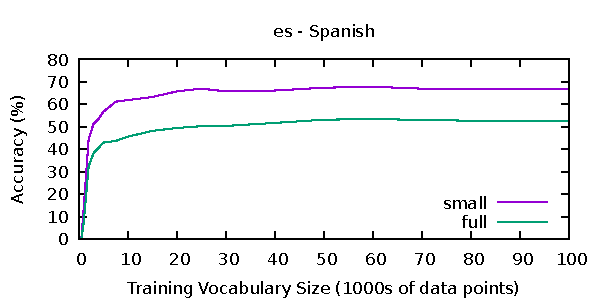
\includegraphics[width=\columnwidth]{fig/dictsize-es.pdf}
    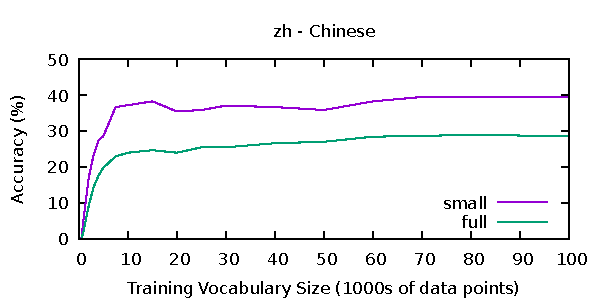
\includegraphics[width=\columnwidth]{fig/dictsize-zh.pdf}
    \caption{BLI accuracy as a function of dataset size.}
    \label{fig:dictsize}
\end{figure}


The goal of this experiment is to measure the effect of training dataset size on the performance of supervised BLI models.
There are two reasons for performing this experiment.
The first is computational.
The runtime and memory usage of most BLI training algorithms is proportional to the input training set size.
So for languages with large training sets, we want to learn at what size should we truncate the dataset in order to speed up training without sacrificing performance.
The second reason is statistical.
The size of the training sets we extracted from Wiktionary follow a power law distribution,
with a small number of high-resource languages having many translations,
but most languages having few translations.
We want to understand how having a small training set will effect the BLI performance of these datasets.

To perform the experiment, we construct modified training sets by taking the first $n$ samples from the Wiktionary training set,
where $n$ ranges from 0 to \numprint{100000}.
%Because the training set is ordered according to word frequency,
%this ensures that each of these training sets contains the most high frequency words.
%This is the best-case scenario for training a bilingual map because word vectors for high frequency words tend to be more accurate than those for low frequency words \citep{},
%and so the truncated set of points will be as close to isomorphic as possible \citep{}.
For each truncated training set, we train the supervised VecMap model \citep{artetxe2018generalizing},
and evaluate on both the small and full test sets.
Results are shown in Figure \ref{fig:dictsize} for the Spanish-English and Chinese-English language pairs.
In both cases, BLI accuracy rapidly increases as the number of training samples reaches 5k, and then tapers off.
After 20k training points, there is minimal improvement and the performance occasionally decreases due to statistical randomness.\footnote{Other language pairs are not shown for space reasons, but all had similar results.}
This is consistent with previous findings on the effect of training dataset size using the MUSE dataset \citep{vulic2016role,qiu2018revisiting,glavas2019properly}.

In the experiments below, we will train many models.
For computational reasons, we truncate the training set size to 20k and expect not to lose any accuracy.
We also know that if we observe extremely poor BLI performance in an experiment with at least (about) 5k entries in the BLI training set,
then the poor performance is likely not explained by the size of the BLI training set but by some other cause.

\subsection{MUSE Corpus vs Wiktionary Corpus}
\label{sec:muse}

Our next experiment attempts to measure the quality of the MUSE and Wiktionary datasets for the 45 language pairs supported by both datasets.
The first three columns of Table \ref{table:muse} show summary statistics of both datasets (details are provided in the table caption).
The fourth column is the most interesting, and is the focus of our explanation here.

We train the VecMap \citep{artetxe2018generalizing} BLI model on each language pair,
once on the MUSE dataset and once on the Wiktionary dataset.
Then for both models, we evaluate on the Wiktionary dataset.
The results are shown in the rightmost column of Table \ref{table:muse}.
Surprisingly, the MUSE training set outperforms the Wiktionary training set for 22/45 of the languages despite coming from a seemingly different distribution.
This suggests that despite the high quality nature of the Wiktionary test set data,
it is not complete,
and more data from more data sources could still be used to improve the alignment of vector spaces.

We hypothesize two reasons to explain this effect.
First, the effect only happens when the MUSE training set is much larger than the Wiktionary training set.
For example, in the case of Slovak, the MUSE training set has \numprint{36891} data points and the Wiktionary set has only \numprint{5396}.
The experiments in Section \ref{sec:dictsize} above suggest that our Wiktionary dataset's size of about 5k words is large enough to get meaningful results, but that a larger dictionary would still improve performance.
Second, Wiktionary is naturally biased towards containing the "dictionary" (i.e.\ unconjugated) forms of words.
 Slovak is a fusional language with many inflected forms for each word, and this helps explain the smaller size of the wiktionary dataset.

\ignore{
Directly comparing the quality of these datasets is difficult to do because there is no ground truth measure available.
Table \ref{table:muse}

Therefore, we create 4 proxies for quality, each with their own advantages and disadvantages, which we describe below.
We conclude that for 23/45 languages, the Wiktionary dataset is clearly superior;
for the remaining 22/45, there is not enough evidence to determine which is superior.
%We do this by training models on both the MUSE and Wiktionary test sets, and then evaluating the models

\textit{Proxy 1: Full Vocab Size.}
Our first proxy is simply the size of the dataset.
Table \ref{table:muse} (column pair 1) shows that 35 of the language pairs have more training data in the MUSE set,
and only 10 language pairs have more training data in the Wiktionary dataset.
As we have seen in Figure \ref{fig:th-vi}, however, we have good reason to be suspicious of the quality of words in the MUSE set.

\textit{Proxy 2: Fraction Distinct.}
One of the major limitations of the MUSE dataset is that it contains many entries where the source and target words are the same in both languages.
This is appropriate for cognate words in the languages, but most of these duplicated entries in the MUSE dataset are not cognates.
In Figure \ref{fig:th-vi}, for example, we see that many of the duplicates are proper nouns (e.g.\ annie, turing, handel), English words incorrectly identified as the foreign language (e.e.\ piston), and html/css/javascript code that accidentally made it into the dataset (e.g.\ getparent, efm, bdfutbol).
For this proxy, we compute the total fraction of words that are distinct between the source and target languages.
The results are shown in Table \ref{table:muse} (column pair 2).
Many of the MUSE datasets have extremely small number of unique words.
This is especially true for low resource languages (e.g.\ Catalan: 0.30, Indonesian: 0.30, Thai: 0.38, Tagalog: 0.28) where the machine translation system used to generate the dataset is likely to have been trained on small datasets.
Remarkably, this is true even for several high resource languages (e.g.\ French: 0.35, Italian: 0.40).
Both of these high resource languages have a large number of cognates with English,
but having more than half the dictionary be identical is clearly inappropriate.
Manual inspection of these datasets indicate that the duplicates are not due to cognates, but due to nonsense words (e.g.\ cjb, bloss, kissling) produced by the machine translation system.
In the Wiktionary dataset, all 45 languages have a higher fraction of distinct words,
and the human curated nature of the dataset ensures that all of the duplicated words are legitimate cognates and not artifacts of a machine translation procedure.

\textit{Proxy 3: Distinct Vocab Size.}
Proxy 1 focused on the quantity of words and proxy 2 focused on the quality;
this proxy is a combined measure of both quantity and quality.
In particular, we compute the total number of words in each dataset that have different source/target pairs.
The results are shown in Table \ref{table:muse} (column pair 3).
When counting the total number of words, only 10 languages had larger datasets in the Wiktionary dataset;
but when counting distinct total words, the number jumps to 21.
Of the remaining languages with larger datasets in the MUSE dataset,
most of these languages are highly inflectional.
By construction, the wiktionary dataset is restricted to lemma forms of words,
but the MUSE set has no such restriction.

\textit{Proxy 4: BLI Accuracy.}

We next remove training data points from both datasets where the source and target language words are the same.
Table \ref{table:muse} (column pair 2) shows that
We next compute the fraction of words in each language where the source and target strings are distinct.
For the Wiktionary dataset, the German and Danish languages have the largest fraction of identical 

Finally, we train VecMap models on the MUSE and Wiktionary datasets, and evaluate them both on the full Wiktionary test set.
}

%%%%%%%%%%%%%%%%%%%%%%%%%%%%%%%%%%%%%%%%
\subsection{The \citet{grave2018learning} Languages}
\label{sec:157}

\citet{grave2018learning} released word vectors in 157 languages trained on the common crawl corpus (a multi-petabyte collection of webpages).
All 45 of the languages in the MUSE corpus studied above appear in the \citet{grave2018learning} corpus;
so in this section we focus on the 112 languages that do not.
As far as we are aware, no one has previously attempted to align these embeddings,
and there are no previously published datasets of bilingual lexicons suitable for training or evaluation.
The Wiktionary corpus is therefore the first publicly available dataset for training and testing alignment models in these languages.
The size of each language's dataset and the accuracy for each model on the small and full test set are shown in Table \ref{table:157}.

We train 3 alignment models on each language:
the Procrustes \citep{xing2015normalized} and Bootstrap Procrustes \citep{glavas2019properly,vulic2019we} as implemented by the MUSE project, %\footnote{\url{https://github.com/facebookresearch/MUSE}},
and VecMap \citep{artetxe2018generalizing}.
%We select these models because they are computationally efficient and do not require expensive hyperparameter tuning (like the RCSLS model of \citet{couling2018loss} does).
There are many other supervised methods and unsupervised methods that would be interesting to train on these datasets,
but we did not have the computational resources to do so.
Thirteen languages achieve an accuracy on the full test set greater than 30: Esperanto (50.00), Galician (46.62), Armenian (39.15), Azerbaijani (37.38), Georgian (37.30), Austurian (36.92), Basque (36.32), Belarusian (35.75), Welsh (34.84), Malayalam (33.62), Serbo-Croatian (33.17), Norwegian Nynorsk (32.35), and Serbian (30.76).
An additional 2 languages achieve an accuracy on the small test set greater than 30: Urdu (37.08) and Mongolian (31.38).
We call out the 30\% threshold in particular because these languages achieve competitive performance with the languages from the widely used MUSE test set (Table \ref{table:muse}),
and therefore are good candidates for downstream applications.
Because of the careful construction of the test set, as described in Section \ref{sec:train-test} above, it is reasonable to compare the absolute performance between languages.
Such comparisons were not recommended for the MUSE dataset \citep{kementchedjhieva2019lost} due to the high variability in quality and content between languages.

We observe that the higher-resource languages (top of table) tend to have better BLI performance than the lower resource languages (bottom of table).
We suggest that this difference is not due to a lower quality of the Wiktionary lexicons,
but to the lower quality of the \citet{grave2018learning} word vectors trained on smaller datasets.
We note that in our dictionary size experiment from Section \ref{sec:dictsize} above,
training lexicons as small as 5k examples give strong performance when the monolingual word vectors are high quality.
In Table \ref{table:157}, however, we see performance drop off long before this 5k mark.
This is particularly notable in the Latin and Sanskrit languages.
Both languages have a large Wiktionary dataset (\numprint{41278} and \numprint{11363}),
but poor BLI performance (13.03 and 2.98 on the full test set).
We attribute this to the fact that these languages are of particular interest to the Wiktionary community for their historical importance, and thus have a lot of entries;
but their historical nature also means there are few webpages written in these languages,
and so the word vectors trained on the common crawl corpus will be of low quality.
%but they are not widely spoken, and so rare in the common crawl corpus, and therefore have poor monolingual word vectors.
Word vectors trained on small corpuses are known to be less stable \citep{pierrejean2018towards,
%antoniak2018evaluating,
wendlandt2018factors,leszczynski2020understanding,burdick2020analyzing} and therefore difficult to align even with large BLI training data \citep{vulic2020all}.

%Another trend we observe is that the more complicated VecMap algorithm tends to perform the best for the high-resource languages (top of the table),
%but the simpler Procrustes algorithm performs best on low-resource languages (bottom of the table).
%We don't have a theoretical justification as for why.

\begin{table*}
    \centering
    \small
    
\begin{tabular}{rlrrcrrcrrcrr}
\toprule
&& \multicolumn{2}{c}{Full Vocab Size} && \multicolumn{2}{c}{Fraction Distinct} && \multicolumn{2}{c}{Distinct Vocab Size} && \multicolumn{2}{c}{BLI Accuracy} \\
\cmidrule[\heavyrulewidth]{3-4}
\cmidrule[\heavyrulewidth]{6-7}
\cmidrule[\heavyrulewidth]{9-10}
\cmidrule[\heavyrulewidth]{12-13}
\multicolumn{2}{l}{Source Language} & MUSE & Wikt && MUSE & Wikt && MUSE & Wikt && MUSE & Wikt \\
\midrule

\texttt{af}  &                                 Afrikaans         &  \textbf{\numprint{37421}}   &  \numprint{4848}             &   ~   &  0.30           &   \textbf{0.95}           &  ~              &   \textbf{\numprint{11226}}  &  \numprint{4605}             &~&  \textbf{  {42.13}}  &                 {35.08}  \\
\texttt{ar}  &                                 Arabic            &  \textbf{\numprint{31355}}   &  \numprint{26361}            &   ~   &  \textbf{1.00}  &   \textbf{1.00}           &  ~              &   \textbf{\numprint{31355}}  &  \numprint{26361}            &~&  \textbf{  {31.94}}  &                 {30.35}  \\
\texttt{bg}  &                                 Bulgarian         &  \textbf{\numprint{55170}}   &  \numprint{13827}            &   ~   &  \textbf{1.00}  &   \textbf{1.00}           &  ~              &   \textbf{\numprint{55170}}  &  \numprint{13827}            &~&  {48.91}   &         \textbf{{52.84}}  \\
\texttt{bn}  &                                 Bengali           &  \textbf{\numprint{23829}}   &  \numprint{5712}             &   ~   &  \textbf{1.00}  &   \textbf{1.00}           &  ~              &   \textbf{\numprint{23829}}  &  \numprint{5712}             &~&  \textbf{  {28.34}}  &                 {26.68}  \\
\texttt{bs}  &                                 Bosnian    &  \numprint{43318}            &  \textbf{\numprint{73449}}   &   ~   &  0.38           &   \textbf{0.99}           &  ~              &   \numprint{16460}           &  \textbf{\numprint{72714}}   &~&  \textbf{  {35.95}}  &                 {29.49}  \\
\texttt{ca}  &                                 Catalan           &  \numprint{78081}            &  \textbf{\numprint{116348}}  &   ~   &  0.30           &   \textbf{0.99}           &  ~              &   \numprint{23424}           &  \textbf{\numprint{115184}}  &~&  \textbf{  {49.79}}  &                 {49.53}  \\
\texttt{cs}  &                                 Czech             &  \textbf{\numprint{64211}}   &  \numprint{35879}            &   ~   &  0.55           &   \textbf{0.98}           &  ~              &   \textbf{\numprint{35316}}  &  \numprint{35161}            &~&  {47.78}   &         \textbf{{49.67}}  \\
\texttt{da}  &                                 Danish            &  \textbf{\numprint{81959}}   &  \numprint{16680}            &   ~   &  0.46           &   \textbf{0.94}           &  ~              &   \textbf{\numprint{37701}}  &  \numprint{15679}            &~&  {49.79}   &         \textbf{{53.56}}  \\
\texttt{de}  &                                 German            &  \textbf{\numprint{101997}}  &  \numprint{68029}            &   ~   &  0.52           &   \textbf{0.94}           &  ~              &   \numprint{53038}           &  \textbf{\numprint{63947}}   &~&  {47.46}   &         \textbf{{48.88}}  \\
\texttt{el}  &                                 Greek             &  \textbf{\numprint{45515}}   &  \numprint{32519}            &   ~   &  \textbf{1.00}  &   \textbf{1.00}           &  ~              &   \textbf{\numprint{45515}}  &  \numprint{32519}            &~&  {53.02}   &         \textbf{{55.45}}  \\
\texttt{es}  &                                 Spanish           &  \textbf{\numprint{112583}}  &  \numprint{91066}            &   ~   &  0.45           &   \textbf{0.95}           &  ~              &   \numprint{50662}           &  \textbf{\numprint{86512}}   &~&  {54.40}   &         \textbf{{54.67}}  \\
\texttt{et}  &                                 Estonian          &  \textbf{\numprint{32776}}   &  \numprint{6901}             &   ~   &  0.64           &   \textbf{0.98}           &  ~              &   \textbf{\numprint{20976}}  &  \numprint{6762}             &~&  \textbf{  {50.04}}  &                 {48.07}  \\
\texttt{fa}  &                                 Persian           &  \textbf{\numprint{41321}}   &  \numprint{14238}            &   ~   &  \textbf{1.00}  &   \textbf{1.00}           &  ~              &   \textbf{\numprint{41321}}  &  \numprint{14238}            &~&  {37.39}   &         \textbf{{39.40}}  \\
\texttt{fi}  &                                 Finnish           &  \numprint{43102}            &  \textbf{\numprint{105030}}  &   ~   &  0.62           &   \textbf{0.99}           &  ~              &   \numprint{26723}           &  \textbf{\numprint{103979}}  &~&  \textbf{  {43.90}}  &                 {43.11}  \\
\texttt{fr}  &                                 French            &  \textbf{\numprint{113324}}  &  \numprint{78837}            &   ~   &  0.35           &   \textbf{0.90}           &  ~              &   \numprint{39663}           &  \textbf{\numprint{70953}}   &~&  \textbf{  {53.92}}  &                 {53.57}  \\
\texttt{he}  &                                 Hebrew            &  \textbf{\numprint{45679}}   &  \numprint{12234}            &   ~   &  \textbf{1.00}  &   \textbf{1.00}           &  ~              &   \textbf{\numprint{45679}}  &  \numprint{12234}            &~&  {33.47}   &         \textbf{{35.32}}  \\
\texttt{hi}  &                                 Hindi             &  \textbf{\numprint{31046}}   &  \numprint{21887}            &   ~   &  \textbf{1.00}  &   \textbf{1.00}           &  ~              &   \textbf{\numprint{31046}}  &  \numprint{21887}            &~&  {33.99}   &         \textbf{{38.28}}  \\
\texttt{hr}  &                                 Croatian    &  \numprint{56424}            &  \textbf{\numprint{73449}}   &   ~   &  0.49           &   \textbf{0.99}           &  ~              &   \numprint{27647}           &  \textbf{\numprint{72714}}   &~&  \textbf{  {47.57}}  &                 {45.21}  \\
\texttt{hu}  &                                 Hungarian         &  \textbf{\numprint{42823}}   &  \numprint{34569}            &   ~   &  0.62           &   \textbf{0.99}           &  ~              &   \numprint{26550}           &  \textbf{\numprint{34223}}   &~&  {45.48}   &         \textbf{{49.29}}  \\
\texttt{id}  &                                 Indonesian        &  \textbf{\numprint{96518}}   &  \numprint{12269}            &   ~   &  0.30           &   \textbf{0.97}           &  ~              &   \textbf{\numprint{28955}}  &  \numprint{11900}            &~&  {35.20}   &         \textbf{{40.15}}  \\
\texttt{it}  &                                 Italian           &  \numprint{103613}           &  \textbf{\numprint{119697}}  &   ~   &  0.40           &   \textbf{0.98}           &  ~              &   \numprint{41445}           &  \textbf{\numprint{117303}}  &~&  \textbf{  {46.43}}  &                 {45.47}  \\
\texttt{ja}  &                                 Japanese          &  \numprint{25969}            &  \textbf{\numprint{73669}}   &   ~   &  \textbf{1.00}  &   \textbf{1.00}           &  ~              &   \numprint{25969}           &  \textbf{\numprint{73669}}   &~&  \textbf{  {24.96}}  &                 {24.96}  \\
\texttt{ko}  &                                 Korean            &  \numprint{20549}            &  \textbf{\numprint{34739}}   &   ~   &  \textbf{1.00}  &   \textbf{1.00}           &  ~              &   \numprint{20549}           &  \textbf{\numprint{34739}}   &~&  {23.84}   &         \textbf{{31.64}}  \\
\texttt{lt}  &                                 Lithuanian        &  \textbf{\numprint{33435}}   &  \numprint{6270}             &   ~   &  0.55           &   \textbf{1.00}           &  ~              &   \textbf{\numprint{18389}}  &  \numprint{6270}             &~&  \textbf{  {51.22}}  &                 {49.86}  \\
\texttt{lv}  &                                 Latvian           &  \textbf{\numprint{46385}}   &  \numprint{14428}            &   ~   &  0.72           &   \textbf{1.00}           &  ~              &   \textbf{\numprint{33397}}  &  \numprint{14428}            &~&  {50.11}   &         \textbf{{52.12}}  \\
\texttt{mk}  &                                 Macedonian        &  \textbf{\numprint{43935}}   &  \numprint{41054}            &   ~   &  \textbf{1.00}  &   \textbf{1.00}           &  ~              &   \textbf{\numprint{43935}}  &  \numprint{41054}            &~&  {37.97}   &         \textbf{{40.23}}  \\
\texttt{ms}  &                                 Malay             &  \textbf{\numprint{73092}}   &  \numprint{5821}             &   ~   &  0.23           &   \textbf{0.97}           &  ~              &   \textbf{\numprint{16811}}  &  \numprint{5646}             &~&  {27.60}   &         \textbf{{28.56}}  \\
\texttt{nl}  &                                 Dutch             &  \textbf{\numprint{93853}}   &  \numprint{67309}            &   ~   &  0.38           &   \textbf{0.97}           &  ~              &   \numprint{35664}           &  \textbf{\numprint{65289}}   &~&  \textbf{  {39.78}}  &                 {36.57}  \\
\texttt{no}  &                                 Norwegian Bokmål  &  \textbf{\numprint{75171}}   &  \numprint{21386}            &   ~   &  0.37           &   \textbf{0.95}           &  ~              &   \textbf{\numprint{27813}}  &  \numprint{20316}            &~&  \textbf{  {54.24}}  &                 {43.96}  \\
\texttt{pl}  &                                 Polish            &  \textbf{\numprint{73901}}   &  \numprint{66225}            &   ~   &  0.48           &   \textbf{0.98}           &  ~              &   \numprint{35472}           &  \textbf{\numprint{64900}}   &~&  \textbf{  {44.18}}  &                 {41.11}  \\
\texttt{pt}  &                                 Portuguese        &  \textbf{\numprint{108686}}  &  \numprint{55927}            &   ~   &  0.42           &   \textbf{0.95}           &  ~              &   \numprint{45648}           &  \textbf{\numprint{53130}}   &~&  {58.42}   &         \textbf{{58.68}}  \\
\texttt{ro}  &                                 Romanian          &  \textbf{\numprint{80821}}   &  \numprint{65122}            &   ~   &  0.39           &   \textbf{0.93}           &  ~              &   \numprint{31520}           &  \textbf{\numprint{60563}}   &~&  \textbf{  {48.96}}  &                 {48.58}  \\
\texttt{ru}  &                                 Russian           &  \numprint{48714}            &  \textbf{\numprint{70740}}   &   ~   &  \textbf{1.00}  &   \textbf{1.00}           &  ~              &   \numprint{48714}           &  \textbf{\numprint{70740}}   &~&  \textbf{  {46.99}}  &                 {39.86}  \\
\texttt{sk}  &                                 Slovak            &  \textbf{\numprint{65878}}   &  \numprint{5681}             &   ~   &  0.56           &   \textbf{0.95}           &  ~              &   \textbf{\numprint{36891}}  &  \numprint{5396}             &~&  \textbf{  {54.29}}  &                 {53.27}  \\
\texttt{sl}  &                                 Slovene           &  \textbf{\numprint{62890}}   &  \numprint{4401}             &   ~   &  0.53           &   \textbf{0.99}           &  ~              &   \textbf{\numprint{33331}}  &  \numprint{4356}             &~&  \textbf{  {49.40}}  &                 {40.86}  \\
\texttt{sq}  &                                 Albanian          &  \textbf{\numprint{52090}}   &  \numprint{8628}             &   ~   &  0.53           &   \textbf{1.00}           &  ~              &   \textbf{\numprint{27607}}  &  \numprint{8628}             &~&  \textbf{  {36.97}}  &                 {33.47}  \\
\texttt{sv}  &                                 Swedish           &  \textbf{\numprint{82348}}   &  \numprint{27724}            &   ~   &  0.42           &   \textbf{0.95}           &  ~              &   \textbf{\numprint{34586}}  &  \numprint{26337}            &~&  {49.12}   &         \textbf{{52.82}}  \\
\texttt{ta}  &                                 Tamil             &  \textbf{\numprint{21230}}   &  \numprint{8376}             &   ~   &  \textbf{1.00}  &   \textbf{1.00}           &  ~              &   \textbf{\numprint{21230}}  &  \numprint{8376}             &~&  \textbf{  {29.11}}  &                 {21.20}  \\
\texttt{th}  &                                 Thai              &  \textbf{\numprint{25332}}   &  \numprint{19988}            &   ~   &  0.38           &   \textbf{1.00}           &  ~              &   \numprint{9626}            &  \textbf{\numprint{19988}}   &~&  {19.70}   &         \textbf{{23.33}}  \\
\texttt{tl}  &                                 Tagalog           &  \textbf{\numprint{34984}}   &  \numprint{17817}            &   ~   &  0.28           &   \textbf{0.98}           &  ~              &   \numprint{9795}            &  \textbf{\numprint{17460}}   &~&  {28.24}   &         \textbf{{30.14}}  \\
\texttt{tr}  &                                 Turkish           &  \textbf{\numprint{68611}}   &  \numprint{15271}            &   ~   &  0.42           &   \textbf{0.98}           &  ~              &   \textbf{\numprint{28816}}  &  \numprint{14965}            &~&  {34.51}   &         \textbf{{40.49}}  \\
\texttt{uk}  &                                 Ukrainian         &  \textbf{\numprint{40723}}   &  \numprint{16910}            &   ~   &  \textbf{1.00}  &   \textbf{1.00}           &  ~              &   \textbf{\numprint{40723}}  &  \numprint{16910}            &~&  {59.10}   &         \textbf{{59.18}}  \\
\texttt{vi}  &                                 Vietnamese        &  \textbf{\numprint{76364}}   &  \numprint{9708}             &   ~   &  0.08           &   \textbf{1.00}           &  ~              &   \numprint{6109}            &  \textbf{\numprint{9708}}    &~&  {11.34}   &         \textbf{{12.34}}  \\
\texttt{zh}  &                                 Chinese           &  \numprint{21597}            &  \textbf{\numprint{119459}}  &   ~   &  \textbf{1.00}  &   \textbf{1.00}           &  ~              &   \numprint{21597}           &  \textbf{\numprint{119459}}  &~&  {24.66}   &         \textbf{{27.78}}  \\
\midrule     \multicolumn{2}{l}{\textbf{Total  Best}}            &  \textbf{\numprint{35}}      &  \numprint{10}               &&  14  &  \textbf{45}    &&  \textbf{\numprint{24}}  &  \numprint{21}  &&  {22}                       &  \textbf{{23}}\\
\bottomrule\end{tabular}


    \caption{
        A comparison of the MUSE and Wiktionary datasets.
        The ``Full Vocab Size'' measures the total number of source/target word pairs in each dataset.
        Recall, however, that the MUSE dataset is machine translated, and has many artifacts from this process.
        One such artifact is the presence of many duplicate entries where the source and target words are the same,
        and frequently not valid words in either language (See Figure \ref{fig:th-vi} for examples in Thai).
        The ``Fraction Distinct'' column measures the fraction of source/target word pairs where the source value does not equal the target.
        This number is extremely low for many of the MUSE lexicons (e.g. 0.38 for Thai and 0.08 for Vietnamese) due to the machine translation generation process.
        This number is high for all of the Wiktionary lexicons because they are sourced from high quality human generated translations.
        All of the duplicate entries are the result of true cognate words between the source language and English.
        The ``Distinct Vocab Size'' column computes the total number of distinct source/target pairs in each lexicon,
        and is equal to the Full Vocab Size column times the Fraction Distinct column.
        We see that many of the MUSE lexicons are still larger than the Wiktionary lexicons because they allow conjugates of words to appear in a lexicon multiple times, but this does not happen in the Wiktionary lexicon.
        Finally the ``BLI Accuracy'' column presents the result of a MUSE-trained model and a Wiktionary trained model on the Wiktionary test set.
        See Section \ref{sec:muse} for details.
    }
    \label{table:muse}
\end{table*}

\begin{table*}
    \centering
    \small
    
\begin{tabular}{rllrcrrrcrrr}
\toprule
&&&&& \multicolumn{3}{c}{Small Test Set} && \multicolumn{3}{c}{Full Test Set} \\
\cmidrule[\heavyrulewidth]{6-8}
\cmidrule[\heavyrulewidth]{10-12}
Rank & \multicolumn{2}{l}{Source Language} & Vocab Size & & Proc & Proc-B & VecMap && Proc & Proc-B & VecMap \\
\midrule

1    &  \texttt{sr}   &  Serbian  &         \numprint{73449}  &                 ~  &  28.51           &              \textbf{47.79}  &               42.57           &               ~  &  19.43           &              \textbf{30.76}  &               29.27           \\
2    &  \texttt{sh}   &  Serbo-Croatian  &         \numprint{73449}  &                 ~  &  42.34           &              \textbf{52.42}  &               46.37           &               ~  &  28.64           &              \textbf{33.17}  &               31.78           \\
3    &  \texttt{la}   &  Latin           &         \numprint{41278}  &                 ~  &  14.11           &              14.11           &               \textbf{21.37}  &               ~  &  9.65            &              9.65            &               \textbf{13.03}  \\
4    &  \texttt{ga}   &  Irish           &         \numprint{26579}  &                 ~  &  24.79           &              24.79           &               \textbf{29.75}  &               ~  &  16.20           &              16.20           &               \textbf{18.81}  \\
5    &  \texttt{hy}   &  Armenian        &         \numprint{22748}  &                 ~  &  50.00           &              \textbf{52.02}  &               50.40           &               ~  &  37.91           &              38.10           &               \textbf{39.15}  \\
6    &  \texttt{nn}   &  Norwegian       Nynorsk   &                 \numprint{19881}  &  ~  &               26.53          &               26.53           &               \textbf{28.98}  &  ~  &               30.17          &               30.17           &               \textbf{33.25}  \\
7    &  \texttt{is}   &  Icelandic       &         \numprint{19570}  &                 ~  &  32.52           &              36.59           &               \textbf{39.43}  &               ~  &  29.82           &              29.91           &               \textbf{34.59}  \\
8    &  \texttt{gl}   &  Galician        &         \numprint{19155}  &                 ~  &  47.77           &              \textbf{52.63}  &               51.82           &               ~  &  45.06           &              45.32           &               \textbf{46.62}  \\
9    &  \texttt{ka}   &  Georgian        &         \numprint{18898}  &                 ~  &  36.71           &              36.71           &               \textbf{42.19}  &               ~  &  34.14           &              34.14           &               \textbf{37.30}  \\
10   &  \texttt{eo}   &  Esperanto       &         \numprint{18534}  &                 ~  &  49.36           &              49.36           &               \textbf{54.94}  &               ~  &  47.14           &              47.14           &               \textbf{50.00}  \\
11   &  \texttt{te}   &  Telugu          &         \numprint{13289}  &                 ~  &  14.11           &              14.11           &               \textbf{15.77}  &               ~  &  13.81           &              13.81           &               \textbf{16.19}  \\
12   &  \texttt{gd}   &  Scottish        Gaelic    &                 \numprint{12443}  &  ~  &               9.80           &               9.80            &               \textbf{11.84}  &  ~  &               8.32           &               8.32            &               \textbf{8.53}   \\
13   &  \texttt{km}   &  Khmer           &         \numprint{11378}  &                 ~  &  21.54           &              \textbf{26.42}  &               22.76           &               ~  &  16.28           &              17.56           &               \textbf{18.50}  \\
14   &  \texttt{sa}   &  Sanskrit        &         \numprint{11363}  &                 ~  &  \textbf{4.08}   &              4.08            &               1.22            &               ~  &  \textbf{2.98}   &              2.98            &               1.56            \\
15   &  \texttt{kk}   &  Kazakh          &         \numprint{11323}  &                 ~  &  \textbf{26.67}  &              26.67           &               23.33           &               ~  &  27.11           &              27.11           &               \textbf{27.20}  \\
16   &  \texttt{ceb}  &  Cebuano         &         \numprint{10853}  &                 ~  &  \textbf{5.88}   &              5.88            &               5.88            &               ~  &  \textbf{8.22}   &              8.22            &               3.88            \\
17   &  \texttt{az}   &  Azerbaijani     &         \numprint{10713}  &                 ~  &  37.65           &              \textbf{39.27}  &               38.46           &               ~  &  36.09           &              \textbf{37.38}  &               37.12           \\
18   &  \texttt{azb}  &  Southern Azerbaijani     &         \numprint{10713}  &                 ~  &  \textbf{2.10}   &              2.10            &               1.40            &               ~  &  \textbf{2.91}   &              2.91            &               1.82            \\
19   &  \texttt{cy}   &  Welsh           &         \numprint{10459}  &                 ~  &  40.57           &              \textbf{46.31}  &               44.26           &               ~  &  30.98           &              34.34           &               \textbf{34.84}  \\
20   &  \texttt{io}   &  Ido             &         \numprint{8127}   &                 ~  &  \textbf{14.00}  &              14.00           &               14.00           &               ~  &  12.30           &              12.30           &               \textbf{12.75}  \\
21   &  \texttt{gv}   &  Manx            &         \numprint{8105}   &                 ~  &  \textbf{5.93}   &              5.93            &               3.39            &               ~  &  \textbf{6.39}   &              6.39            &               3.27            \\
22   &  \texttt{mt}   &  Maltese         &         \numprint{8089}   &                 ~  &  \textbf{0.00}   &              0.00            &               0.00            &               ~  &  \textbf{0.00}   &              0.00            &               0.00            \\
23   &  \texttt{ml}   &  Malayalam       &         \numprint{7465}   &                 ~  &  27.78           &              28.63           &               \textbf{30.34}  &               ~  &  29.60           &              32.47           &               \textbf{33.62}  \\
24   &  \texttt{lb}   &  Luxembourgish   &         \numprint{7438}   &                 ~  &  4.88            &              \textbf{8.54}   &               5.69            &               ~  &  10.89           &              \textbf{11.99}  &               6.13            \\
25   &  \texttt{sw}   &  Swahili         &         \numprint{7324}   &                 ~  &  12.45           &              12.86           &               \textbf{15.35}  &               ~  &  15.94           &              \textbf{18.01}  &               17.49           \\
26   &  \texttt{ur}   &  Urdu            &         \numprint{7013}   &                 ~  &  26.25           &              \textbf{37.08}  &               26.25           &               ~  &  23.64           &              \textbf{29.73}  &               24.81           \\
27   &  \texttt{yi}   &  Yiddish         &         \numprint{6869}   &                 ~  &  4.86            &              4.86            &               \textbf{5.26}   &               ~  &  7.79            &              7.79            &               \textbf{9.79}   \\
28   &  \texttt{my}   &  Burmese         &         \numprint{5902}   &                 ~  &  13.52           &              \textbf{16.80}  &               13.11           &               ~  &  13.77           &              \textbf{15.90}  &               15.26           \\
29   &  \texttt{ast}  &  Asturian        &         \numprint{5645}   &                 ~  &  27.98           &              30.86           &               \textbf{33.33}  &               ~  &  30.12           &              33.65           &               \textbf{36.92}  \\
30   &  \texttt{bcl}  &  Bikol           Central   &                 \numprint{5069}   &  ~  &               \textbf{6.22}  &               6.22            &               4.98            &  ~  &               \textbf{5.16}  &               5.16            &               3.53            \\
31   &  \texttt{be}   &  Belarusian      &         \numprint{4598}   &                 ~  &  27.92           &              \textbf{30.00}  &               27.92           &               ~  &  32.81           &              \textbf{35.75}  &               33.92           \\
32   &  \texttt{mn}   &  Mongolian       &         \numprint{4470}   &                 ~  &  21.34           &              \textbf{31.38}  &               19.67           &               ~  &  21.10           &              \textbf{27.97}  &               19.14           \\
33   &  \texttt{as}   &  Assamese        &         \numprint{4341}   &                 ~  &  1.28            &              1.28            &               \textbf{1.70}   &               ~  &  4.49            &              4.49            &               \textbf{4.72}   \\
34   &  \texttt{oc}   &  Occitan         &         \numprint{4317}   &                 ~  &  16.96           &              18.70           &               \textbf{20.87}  &               ~  &  20.26           &              \textbf{22.23}  &               22.23           \\
35   &  \texttt{gu}   &  Gujarati        &         \numprint{4068}   &                 ~  &  10.78           &              \textbf{18.53}  &               10.34           &               ~  &  10.85           &              \textbf{16.81}  &               12.51           \\
36   &  \texttt{ba}   &  Bashkir         &         \numprint{4053}   &                 ~  &  7.00            &              7.00            &               \textbf{9.47}   &               ~  &  9.03            &              9.03            &               \textbf{9.54}   \\
37   &  \texttt{sco}  &  Scots           &         \numprint{3734}   &                 ~  &  \textbf{9.09}   &              9.09            &               3.54            &               ~  &  \textbf{10.82}  &              10.82           &               8.19            \\
38   &  \texttt{mg}   &  Malagasy        &         \numprint{3634}   &                 ~  &  \textbf{5.26}   &              5.26            &               4.78            &               ~  &  \textbf{4.05}   &              4.05            &               3.64            \\
39   &  \texttt{vec}  &  Venetian        &         \numprint{3570}   &                 ~  &  \textbf{3.24}   &              3.24            &               2.43            &               ~  &  \textbf{3.94}   &              3.94            &               3.48            \\
40   &  \texttt{yo}   &  Yoruba          &         \numprint{3536}   &                 ~  &  \textbf{1.34}   &              1.34            &               0.00            &               ~  &  \textbf{0.87}   &              0.87            &               0.00            \\
41   &  \texttt{bo}   &  Tibetan         &         \numprint{3438}   &                 ~  &  \textbf{1.02}   &              1.02            &               0.00            &               ~  &  \textbf{1.48}   &              1.48            &               0.00            \\
42   &  \texttt{sah}  &  Yakut           &         \numprint{3265}   &                 ~  &  \textbf{2.87}   &              2.87            &               0.82            &               ~  &  \textbf{4.00}   &              4.00            &               2.83            \\
43   &  \texttt{qu}   &  Quechua         &         \numprint{3190}   &                 ~  &  \textbf{4.13}   &              4.13            &               0.00            &               ~  &  \textbf{3.60}   &              3.60            &               0.00            \\
44   &  \texttt{eu}   &  Basque          &         \numprint{3117}   &                 ~  &  20.89           &              \textbf{38.67}  &               23.56           &               ~  &  25.42           &              \textbf{36.32}  &               23.48           \\
45   &  \texttt{mr}   &  Marathi         &         \numprint{3016}   &                 ~  &  11.02           &              \textbf{22.88}  &               13.98           &               ~  &  13.73           &              \textbf{19.82}  &               12.85           \\
46   &  \texttt{pnb}  &  Western Punjabi         &         \numprint{2692}   &                 ~  &  0.00            &              \textbf{0.52}   &               0.00            &               ~  &  0.00            &              \textbf{0.37}   &               0.00            \\
47   &  \texttt{pa}   &  Punjabi         &         \numprint{2692}   &                 ~  &  \textbf{4.66}   &              4.66            &               2.54            &               ~  &  \textbf{5.35}   &              5.35            &               3.36            \\
48   &  \texttt{vo}   &  Volapük         &         \numprint{2673}   &                 ~  &  \textbf{2.98}   &              2.98            &               0.85            &               ~  &  \textbf{3.92}   &              3.92            &               2.04            \\
49   &  \texttt{ku}   &  Northern        Kurdish   &                 \numprint{2658}   &  ~  &               \textbf{2.87}  &               1.64            &               2.87            &  ~  &               5.52           &               \textbf{5.79}   &               3.77            \\
50   &  \texttt{rm}   &  Romansch        &         \numprint{2479}   &                 ~  &  \textbf{2.03}   &              2.03            &               1.22            &               ~  &  \textbf{5.64}   &              5.64            &               4.05            \\
51   &  \texttt{ia}   &  Interlingua     &         \numprint{2397}   &                 ~  &  7.29            &              \textbf{10.12}  &               4.45            &               ~  &  8.25            &              \textbf{9.68}   &               5.22            \\
52   &  \texttt{ne}   &  Nepali          &         \numprint{2185}   &                 ~  &  7.88            &              \textbf{10.37}  &               2.07            &               ~  &  10.11           &              \textbf{10.51}  &               4.65            \\
53   &  \texttt{fy}   &  West            Frisian   &                 \numprint{2137}   &  ~  &               7.50           &               \textbf{10.83}  &               4.17            &  ~  &               10.48          &               \textbf{14.06}  &               5.41            \\
54   &  \texttt{scn}  &  Sicilian        &         \numprint{2050}   &                 ~  &  \textbf{2.86}   &              2.86            &               1.63            &               ~  &  \textbf{5.41}   &              5.41            &               2.85            \\
55   &  \texttt{ug}   &  Uyghur          &         \numprint{1919}   &                 ~  &  \textbf{1.72}   &              1.72            &               0.00            &               ~  &  \textbf{3.78}   &              3.78            &               0.15            \\
56   &  \texttt{als}  &  Alemannic       German    &                 \numprint{1888}   &  ~  &               \textbf{0.50}  &               0.50            &               0.00            &  ~  &               \textbf{2.64}  &               2.64            &               0.00            \\
57   &  \texttt{uz}   &  Uzbek           &         \numprint{1845}   &                 ~  &  \textbf{8.06}   &              8.06            &               7.11            &               ~  &  \textbf{12.64}  &              12.64           &               8.58            \\
58   &  \texttt{kn}   &  Kannada         &         \numprint{1837}   &                 ~  &  6.19            &              \textbf{20.00}  &               8.10            &               ~  &  9.12            &              \textbf{21.40}  &               7.19            \\
59   &  \texttt{tg}   &  Tajik           &         \numprint{1725}   &                 ~  &  11.79           &              \textbf{18.34}  &               14.69           &               ~  &  \textbf{16.25}  &              0.00            &               0.00            \\
60   &  \texttt{jv}   &  Javanese        &         \numprint{1641}   &                 ~  &  \textbf{0.00}   &              0.00            &               0.00            &               ~  &  \textbf{0.00}   &              0.00            &               0.00            \\

\bottomrule
\end{tabular}


    \caption{
        Results of the experiment described in Section \ref{sec:157}.
        Displayed are results on the languages with the 60 largest lexicons from the \citet{grave2018learning} corpus that are not also included in the MUSE corpus.
    }
    \label{table:157}
\end{table*}

%%%%%%%%%%%%%%%%%%%%%%%%%%%%%%%%%%%%%%%%%%%%%%%%%%%%%%%%%%%%%%%%%%%%%%%%%%%%%%%%
\ignore{
\section{Weaknesses}

Conjugations

French/Chinese wiktionaries use different formats

The formatting is inconsistent, resulting in parse errors
}

\clearpage
\bibliography{anthology,custom}

\appendix

%\section{Example Appendix}
%\label{sec:appendix}
%
%This is an appendix.

\end{document}
